% Canonical entry point for Arithmetic Expression Geometry I.
\documentclass[11pt]{article}

\usepackage[letterpaper,margin=1in]{geometry}
\usepackage[T1]{fontenc}
\usepackage[utf8]{inputenc}
\usepackage[english]{babel}
\usepackage{lmodern}
\usepackage{amsmath,amssymb,amsthm,mathtools}
\usepackage{booktabs,graphicx,microtype,xcolor,tikz,url}
\usetikzlibrary{arrows.meta,positioning,calc}
\usepackage[colorlinks=true,linkcolor=blue!45!black,citecolor=green!35!black,
  urlcolor=blue!55!black,pdfencoding=auto]{hyperref}

\newtheorem{theorem}{Theorem}[section]
\newtheorem{proposition}[theorem]{Proposition}
\newtheorem{lemma}[theorem]{Lemma}
\newtheorem{corollary}[theorem]{Corollary}
\theoremstyle{definition}
\newtheorem{definition}[theorem]{Definition}
\newtheorem{example}[theorem]{Example}
\newtheorem{convention}[theorem]{Convention}
\theoremstyle{remark}
\newtheorem{remark}[theorem]{Remark}
\newtheorem{warning}[theorem]{Warning}

\newcommand{\R}{\mathbb{R}}
\newcommand{\Q}{\mathbb{Q}}
\newcommand{\K}{\mathbb{K}}
\newcommand{\PP}{\mathbb{P}}
\newcommand{\Aff}{\operatorname{Aff}}
\newcommand{\PGL}{\operatorname{PGL}}
\newcommand{\Hist}{\operatorname{Hist}}
\newcommand{\ev}{\operatorname{ev}}
\newcommand{\id}{\operatorname{id}}
\newcommand{\Span}{\operatorname{span}}
\newcommand{\dd}{\,\mathrm{d}}
\newcommand{\Lie}{\mathcal{L}}
\newcommand{\reg}{\mathrm{reg}}
\newcommand{\sing}{\mathrm{sing}}

\title{\textbf{Arithmetic Expression Geometry I: Foundations}\\[0.45em]
\large Sequential and Branching Histories, Order-Topological Calculus, and
Hole--Cap Geometry}
\author{
Mingli Yuan\thanks{Corresponding author and sole holder of scientific
responsibility for this manuscript
(\texttt{mingli@swarma.org}).  Formalization, machine checking, computation,
proof drafting, and writing were assisted by DeepSeek Harness, an
artificial-intelligence research agent (model
\texttt{deepseek-v4-flash-vision-exp}); that assistance is credited on this
title page and in the acknowledgements, but it is not human authorship, since
the agent is not a natural person and cannot sign a copyright transfer or serve
as corresponding author.  Contribution-level provenance is recorded in
\texttt{AUTHORSHIP\_AND\_PROVENANCE.md}.}\\
\small Swarma Research\\
\small Beijing 100083, China\\[0.5em]
\small\itshape with formalization and computational assistance\\
\small\itshape from DeepSeek Harness
(model \texttt{deepseek-v4-flash-vision-exp})
}
\date{September 22, 2026\\[0.25em]
\small Draft manuscript under mathematical review.\\[0.35em]
\small
\textbf{MSC 2020:} 20H10 (primary); 05C05, 58K05;
20G15, 68Q42, 53C21}

\begin{document}
\maketitle

\begin{quote}\small
\textbf{Draft notice.}
This manuscript is a working draft in the editorial and publication sense.
Here ``draft'' is not a mathematical claim-status label and does not alter the
status of any theorem, proposition, computation, conjecture, or open problem.
The geometric chapters that earlier versions of this paper contained are now
developed in Paper~0; the migration is recorded in
\texttt{governance/00b-paper-0-geometric-foundation-amendment.md}.
\end{quote}

\begin{abstract}
Ordinary arithmetic evaluation collapses an expression tree into an endpoint
value and discards the order of the computation.
This paper develops the syntax of that discarded order, its order-topological
and analytic structure, and the zero and hole--cap geometry of the spaces on
which the words act.
A finite binary expression tree has a unique legal internal evaluation order
exactly when its internal dependency poset is a chain, equivalently when its
internal vertices form a single spine; marking an accumulator then makes fully
marked planar trees and chronological words of one-hole contexts correspond
bijectively.  Operand-slot chirality is retained as explicit data, distinct
from planar mirror, temporal reversal, and path inverse.
For a general branching tree the dependency poset carries a down-set
information order whose ideal completion is the dcpo of finite and (finitely
predicated) infinite computation DAGs, and the partial evaluations of a fixed
tree form a finite distributive lattice whose maximal chains are exactly the
spinal histories (Birkhoff duality).
On the continuous lattice $[0,\infty]$, the elementary contexts realize the
Scott and Lawson structure: addition is the way-below witness, scaling is a
Scott automorphism, and the reciprocal is the order-reversing involution whose
adjoining turns the one-sided Scott topology into the two-sided Hausdorff Lawson
topology, mirroring the passage from the positive affine semigroup to
$\mathrm{PGL}_2(\mathbb R)$.
For non-degenerate bilateral contexts over an arbitrary field $K$, projective
evaluation is compatible with chronological composition; the elementary contexts
generate $\mathrm{PGL}_2(K)$, those fixing infinity form the affine sector
$B_\infty\cong\mathrm{Aff}(1,K)$ onto which the affine sublanguage maps
surjectively, and the same case division yields the rank-one Bruhat
decomposition.  Over $\mathbb Q(\sqrt2)$, the three-context sublanguage generated
by $z\mapsto z\pm\sqrt2$ and $z\mapsto-1/z$ realizes the $q=4$ Hecke group, and
the order-four relation $(JT)^4=1$ is carried by an explicit eight-step marked
history that is projectively trivial yet ordinarily inadmissible at
$x=-\sqrt2$; projective non-degeneracy is therefore kept separate from ordinary
admissibility.
The analysis of these histories has three pillars.  The differential pillar
identifies the order defect of the minimal branching DAG $\{\mathrm{add},
\mathrm{multiply}\}$ with the contact curvature $[D_u,D_v]=\mu\lambda\,\partial_a$.
The integral pillar expresses the order defect as a group-valued $1$-cocycle on
the linear-extension graph, closed by the Jacobi identity and by the holographic
Stokes theorem, which pushes the bulk curvature to the boundary holonomy.  The
series pillar expands the history evaluation into the free Lie algebra as a
Magnus series, whose arity-$k$ brackets are carried by the $(k-1)$-cells of the
down-set lattice and whose abelianization is the difference substitution.
On the geometric side, five notions of hole and four of boundary are kept
distinct; a decorated network thickened to a ball-and-tube body exhibits the
hole--disk complementarity ``the surface gives the hole its meaning, the body
gives the disk its meaning'', and a constant-boundary disk admits no regular AES
capping.
An explicit tunnel-drilling model adds a boundary handle and changes a filling
disk into an annulus whose outer edge no longer bounds in the body; a split--merge
DAG realizes the corresponding genus without directed feedback.
In a regular arithmetic expression space, subject to the eikonal
axiom $|\nabla a|_g^2=\mu^2+\lambda^2a^2$ with $\mu\ne0$, the zero locus of the
assignment is a smooth curve with no isolated point, crossing, or branch point;
on a connected, complete, boundaryless space the unit-gradient rectification of
the assignment gives a diffeomorphism $M\cong Z(a)\times\mathbb R$, so branching
zero networks are excluded in the regular category.  Singular arithmetic
expression spaces, whose singular set is closed, nowhere dense, and locally
essential, are then defined, with two essential puncture mechanisms
(non-$C^1$ assignment versus conformal-background degeneration); a disc model
with an isolated non-$C^1$ zero is verified, and parameter families with
spatially regular zeros are shown to have submersive total zero sets under a
stated properness hypothesis.
\end{abstract}

\noindent\textbf{Keywords:}
arithmetic expression geometry; binary expression trees; dependency posets and
linear extensions; one-hole contexts; down-set dcpo and Birkhoff duality;
Scott--Lawson topology; projective linear group; Bruhat decomposition; Hecke
groups; order defect and contact curvature; Magnus series and free Lie algebra;
hole--cap geometry; eikonal equation and zero loci; complete splitting theorem;
singular arithmetic expression spaces

\setcounter{tocdepth}{2}
\tableofcontents
\newpage

\section*{Interface: From Paper 0 to Paper I}
\addcontentsline{toc}{section}{Interface: From Paper 0 to Paper I}
Paper~0 is the geometric foundation of this series.  It constructs the space in
which the elementary arithmetic operations act as motions, the dual reading of
those motions, the commutativization against which their order defect is
measured, and the contact structure of that defect.  It fixes explicit left- and
right-expanded conventions, proves the distributive expansion that relates two
expansions sharing an operator, and treats reciprocals, poles, the projective
point at infinity, affine and reciprocal fixed points, and the common
$2\times2$ matrix representation.

The present paper begins one level earlier and stays there.  Its first problem
is intrinsic: which finite binary expression trees have a unique legal order of
internal evaluation, including mixed operand-slot patterns?  The answer is the
single-spine classification.  Choosing an accumulator then gives the marked
spinal histories used throughout this paper.  We retain that terminology and
formalism unchanged.

The division of labour is therefore the following.
\begin{itemize}
  \item \textbf{Paper 0:} expansions, arithmetic motions, the models
  $\mathfrak E_0$ and $\mathfrak E_1$, ripple geometry, affine cocycles, the
  accumulative commutative space and tearing, and the contact structure of the
  tearing.
  \item \textbf{Paper I:} intrinsic sequential and branching histories, bilateral
  projective evaluation, the Scott--Lawson order topology of histories, the
  analysis three pillars (differential, integral, series), and the hole--cap
  fine geometry of the regular and singular zero theory.
\end{itemize}
Per the amendment recorded in
\path{governance/00d-paper-I-calculus-and-capping-amendment.md}, the analysis
and the hole--cap geometry are now developed \emph{here}; Paper~0's contact,
ACS, and punctured-AES chapters are the canonical upstream, and this paper
restates the specific primitives it needs at the same labels.

This paper imports, with labels and proofs unchanged from Paper~0:
\begin{enumerate}
  \item the regular arithmetic expression space
  $\bigl(M,g,a;\mu,\lambda\bigr)$ and its eikonal axiom
  $|\nabla a|_g^2=\mu^2+\lambda^2 a^2$ with $\mu\ne0$
  (\texttt{def:regular-aes}), together with the canonical arithmetic frame
  (\texttt{prop:canonical-arithmetic-frame});
  \item the arithmetic contact model $\mathcal C=\mathbb R^3_{(u,v,a)}$, the
  contact one-form $\alpha=da-\mu\,du-\lambda a\,dv$
  (\texttt{eq:arithmetic-contact-form}), the horizontal fields
  $D_u=\partial_u+\mu\partial_a$, $D_v=\partial_v+\lambda a\partial_a$
  (\texttt{eq:horizontal-arithmetic-fields}), and the contact curvature bracket
  $[D_u,D_v]=\mu\lambda\,\partial_a$ (\texttt{thm:contact-curvature});
  \item the accumulative commutative space $\mathcal A=\mathbb R^2_{(A,M)}$ and
  the weighted torsion--Stokes theorem (\texttt{thm:torsion-stokes});
  \item the punctured AES (\texttt{def:p0-punctured-aes}) and the two-sided
  collar contract (\texttt{def:p0-collar-contract}).
\end{enumerate}
These imports are restated in the chapters that use them; no theorem of Paper~0
is re-proved here, and the ordinary-admissibility / projective-continuation
distinction remains active throughout.


\section{Introduction}\label{sec:introduction}
% Canonical Paper I source.
An arithmetic expression has several mathematically distinct lives.  It is a finite
syntax tree; it may be equipped with a legal order of evaluation; a chosen running
value turns that order into a marked history; the history induces an operator; and
the operator sends an initial value to an endpoint.  Ordinary arithmetic usually
passes through these levels as quickly as possible.  AEG instead asks what is lost
at each passage.

The guiding structure of this paper is
\begin{equation}\label{eq:process-result-hierarchy}
\begin{gathered}
\text{unmarked sequential tree}
  \xrightarrow{\text{choose an accumulator}}
\text{marked planar sequential tree},\\
\text{marked planar sequential tree}
  \longleftrightarrow
\text{bounded marked history},\\
\text{bounded marked history}
  \longrightarrow \text{operator}
  \longrightarrow \text{endpoint value},\\
\text{bounded marked history}
  \longrightarrow \text{charge shadow}.
\end{gathered}
\end{equation}
The first arrow denotes a choice, not a canonical map.  When the planar structure,
mark, operation labels, constants, and slots are retained, the double arrow is the
bijection proved in Section~\ref{sec:sequential-histories}.  The two arrows leaving a
history are separate forgetful maps: charge is not a function of the evaluated
operator, and an endpoint is not a function of charge alone.  Different histories
may nevertheless induce the same operator, and different operators may agree at one
chosen initial value.  The geometry belongs primarily to these intermediate
levels, before endpoint evaluation has erased the order of construction.

Figure~\ref{fig:process-result-structure} renders this structure explicitly.
It is a map of the distinctions used in the paper, not a claim that any
forgetful arrow is injective.

\begin{figure}[t]
\centering
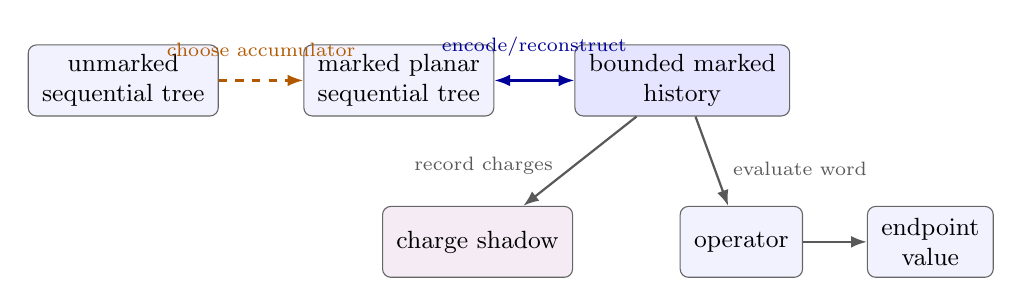
\begin{tikzpicture}[
  stage/.style={draw=black!60,rounded corners=3pt,fill=blue!5,
                minimum height=9mm,align=center,font=\small,inner xsep=5pt},
  forget/.style={-{Latex[length=2mm]},thick,black!65},
  choice/.style={-{Latex[length=2mm]},thick,dashed,orange!70!black},
  bij/.style={{Latex[length=2mm]}-{Latex[length=2mm]},thick,blue!60!black}
]
  \node[stage] (tree) at (-4.5,1.25) {unmarked\\sequential tree};
  \node[stage] (marked) at (-1.0,1.25) {marked planar\\sequential tree};
  \node[stage,fill=blue!10] (history) at (2.6,1.25)
    {bounded marked\\history};
  \node[stage,fill=violet!8] (charge) at (0,-0.8) {charge shadow};
  \node[stage] (operator) at (3.35,-0.8) {operator};
  \node[stage] (endpoint) at (5.75,-0.8) {endpoint\\value};

  \draw[choice] (tree)--node[above=5pt,font=\scriptsize] {choose accumulator} (marked);
  \draw[bij] (marked)--node[above=5pt,font=\scriptsize] {encode/reconstruct} (history);
  \draw[forget] (history)--node[pos=0.58,right=3pt,font=\scriptsize]
    {evaluate word} (operator);
  \draw[forget] (operator)--(endpoint);
  \draw[forget] (history)--node[pos=0.55,left=4pt,font=\scriptsize]
    {record charges} (charge);
\end{tikzpicture}
\caption{The process-to-result structure.  Choosing an accumulator marks an
unmarked sequential tree; a fully marked planar tree and a bounded marked
history determine one another.  From the history, operator evaluation and the
charge map are separate information-losing branches, while an endpoint is
obtained by applying the operator to an initial value.}
\label{fig:process-result-structure}
\end{figure}

\subsection{Sequential histories}

Not every expression tree determines a unique history.  Independent subexpressions
may be evaluated in either order, so a single tree can have many legal linear
extensions of its dependency order.  Section~\ref{sec:sequential-histories} isolates
the precise exception.  For a finite binary tree, uniqueness of the internal
evaluation order is equivalent to the internal vertices forming one chain, or
equivalently one spine.  A marked accumulator on that spine determines a word of
one-hole contexts
\[
 C_{\omega,c}^{(1)}[z]=\omega(z,c),
 \qquad
 C_{\omega,c}^{(2)}[z]=\omega(c,z).
\]
The superscript records the operand slot occupied by the current value.  It is not a
time direction.  This distinction prevents three operations that are often blurred
in informal tree pictures---planar mirror, temporal reversal, and path inverse---from
being identified.

This use of syntax is modest.  Formal generation and rewriting have long histories
in logic and theoretical computer science; classical points of reference include
Post's work on combinatorial reduction and Chomsky's generative hierarchies
\cite{Post1943FormalRO,Chomsky1956ThreeMF}.  Here the purpose is different: the
sequential fragment supplies a controlled domain on which evaluation can be treated
as a path without pretending that every arithmetic tree has a unique path.

\subsection{Why bilateral completion matters}

Earlier affine calculations use the current value in one distinguished operand slot.
That fragment is closed under translations and nonzero scalings and is therefore
naturally represented by the affine group of the line.  Once both operand slots are
allowed, the context $z\mapsto c/z$ introduces inversion.  The correct algebraic
ambient space is then the projective line and its fractional linear transformations.

Section~\ref{sec:projective-affine} records, over an arbitrary field $K$, that the
non-degenerate bilateral contexts generate $\PGL_2(K)$; the generation theorem
itself is proved in Paper~0, and what this paper adds is its reading through the
history language.  The affine transformations
are exactly the stabilizer of the projective point at infinity.  Thus the continuous
geometry is neither discarded nor promoted to the whole theory: it is identified
precisely as the affine sector of a larger projective semantics.  The geometric
reading of these operators --- addition and multiplication as motions of an
arithmetic expression space, and second-slot division as the projective step --- is
developed in Paper~0 and used here only at the operator level.

Inside that larger semantics, the two contexts
\[
  T(z)=z+\sqrt2,
  \qquad
  J(z)=-\frac1z
\]
generate the $q=4$ Hecke group.  Section~\ref{sec:projective-affine} verifies
the relation $(JT)^4=1$ directly from the context matrices and formulates the
resulting interface from arithmetic words to group operators and then to cell
cosets.  This restricted alphabet is important because its hyperbolic
cellulations are produced by arithmetic operator semantics rather than imposed
after endpoint evaluation.  The interface is deliberately not a bijection:
relations identify different histories, and stabilizers identify different
operators at the level of cells or endpoints.

Projective continuation does not repair an inadmissible ordinary computation.  For
example, $c/z$ has a well-defined projective value at $z=0$, namely infinity, while
ordinary division by zero remains undefined.  We keep the ordinary domain and the
projective extension as separate data throughout.

\subsection{Main results}

The first group of results is combinatorial and syntactic.  The trees with a
unique legal internal evaluation order are exactly those whose internal vertices
form a single spine; marking a leaf at the innermost vertex turns such a tree into
a bounded marked spinal history, and the two constructions are mutually inverse
when planar data are retained.  Operand-slot chirality is part of that data and is
kept distinct from chronological direction.

The second group is projective.  The non-degenerate bilateral contexts generate
$\PGL_2(K)$ for every field $K$, the contexts fixing infinity form the affine
sector, and the case division in that generation proof yields the rank-one Bruhat
decomposition.  The generation theorem is Paper~0's, where it is proved for
arbitrary fields; the statement and the Bruhat consequence are repeated here at
the history level because the rest of the paper is written in that language.  The
$\mathbb Q(\sqrt2)$-sublanguage generated by translation by $\sqrt2$ and by
inversion carries the order-four relation $(JT)^4=1$, realized by an explicit
eight-step marked history that is projectively trivial and ordinarily inadmissible
at one initial value.  That example is the reason this paper keeps ordinary
admissibility as a separate hypothesis from projective non-degeneracy.

The third group is the zero theory of regular arithmetic expression spaces.
Section~\ref{sec:regular-aes-interface} restates the definition imported from
Paper~0; Section~\ref{sec:zero-geometry} proves that the zero locus of a regular
assignment is a smooth curve, that a complete connected boundaryless regular AES
splits as $Z(a)\times\mathbb R$, that this forbids branching or multiple zero
components in the regular category, and that a smooth parameter family with
spatially regular zeros has a submersive total zero set --- with the properness
warning that prevents the last statement from being read as triviality.  The
section then defines singular arithmetic expression spaces and verifies one
isolated-zero model in detail.

Everything else that earlier versions of this paper developed --- the two affine
translation coordinates, the continuous arithmetic motion, the basic hyperbolic
model $\mathfrak E_0$, the accumulative commutative space, tearing, and the
contact structure --- now belongs to Paper~0, where it is proved at the same
labels.  This paper cites those results rather than restating them, with the sole
exception of the regular-AES interface needed to state its own zero theorems.

\subsection{Scope and relation to standard geometry}

Several ingredients used here are standard: finite posets and their linear
extensions, fractional linear transformations, and the regular-value theorem.
The mathematical contribution sought in Paper~I is their history-sensitive
arithmetic organization and the exact interfaces among them.

Four boundaries are enforced.  First, the geometric construction of arithmetic
expression spaces, their motions, their commutativization, and their contact
structure belongs to Paper~0.  Second, a horizontal contact distribution does not
by itself select a unique complex structure, so arithmetic holomorphic and
harmonic theories are deferred to Paper II; this includes any automorphic-function
theory built on the $G_4$ action.  Third, the regular-value theorem is only the
starting point for singular families: pulling analytic real loci back to the Hecke
cellulation, and developing their multiple zeros, discriminants, tubes, braids,
and knots, belong to Paper III.  Fourth, projective bivaluations, homogeneous
quotient towers, and condensation belong to Paper IV, and no computational lower
bound follows from noncommutativity or negative curvature alone.

\subsection{Organization}

Section~\ref{sec:sequential-histories} develops sequential trees and marked
histories.  Section~\ref{sec:projective-affine} gives the bilateral projective
semantics and locates the affine sector.
Section~\ref{sec:regular-aes-interface} restates the regular-AES interface
imported from Paper~0.  Section~\ref{sec:zero-geometry} develops the regular and
singular zero geometry.  Section~\ref{sec:conclusion} records what is proved,
what remains open, and the interfaces to the later papers.  The appendices
collect convention checks and the small examples that separate the equality
levels of \eqref{eq:process-result-hierarchy}.

\section{Sequential Arithmetic Histories}\label{sec:sequential-histories}
% Canonical Paper I source.
Arithmetic evaluation is usually presented as a map from a syntactic expression
to its value.  This description suppresses the order in which intermediate
values are formed.  We begin by isolating the finite binary trees for which the
internal operations have only one legal temporal order.  Such a tree is not yet
a history: one must also mark which leaf of its innermost operation is to be
carried forward as the evolving value.  The resulting object, a marked spinal
history, is the syntactic unit used in the remainder of the paper.

Throughout this section, $K$ is a field and
\[
  \Omega=\{+,-,\times,/\}
\]
is the binary arithmetic signature.  Division is interpreted as a partial
operation in ordinary arithmetic.  The combinatorial statements below apply
to any binary signature; the choice of $\Omega$ is needed only when histories
are evaluated.

\subsection{Expression trees and dependency}

\begin{definition}[Arithmetic expression tree]
\label{def:arithmetic-expression-tree}
An \emph{arithmetic expression tree over $K$} is a finite rooted planar binary
tree whose leaves are labelled by elements of $K$ or by formal variables and
whose internal vertices are labelled by elements of $\Omega$.  Its set of
internal vertices is denoted by $I(T)$.
\end{definition}

The planar structure records the first and second operand slots.  It does not,
by itself, specify a temporal order between operations on disjoint subtrees.
That order is recorded by the dependency relation.

\begin{definition}[Internal dependency poset]
\label{def:internal-dependency-poset}
For $u,v\in I(T)$, write $u\preccurlyeq_T v$ when either $u=v$ or the value
produced at $u$ is required as an input at $v$.  Equivalently, $v$ lies on the
path from $u$ to the root.  A \emph{legal internal evaluation order} is a
linear extension of the finite poset $(I(T),\preccurlyeq_T)$.
\end{definition}

Leaves are not included in $I(T)$.  Thus a tree with no internal vertex has the
unique empty internal evaluation order.  This convention separates the order
of operations from the prior availability of atomic inputs.

We shall use the following elementary finite-poset fact in both directions.

\begin{lemma}[Unique linear extensions]
\label{lem:unique-linear-extension}
A finite poset has a unique linear extension if and only if it is a chain.
\end{lemma}

\begin{proof}
Every linear extension of a chain is its given total order, so a chain has a
unique linear extension.  Conversely, let $P$ be a finite poset and suppose
that $u,v\in P$ are incomparable.  Adding the relation $u<v$ and taking its
transitive closure cannot create a directed cycle: such a cycle would contain
a pre-existing path $v\leq u$, contrary to incomparability.  The resulting
finite partial order has a linear extension.  The same argument with $v<u$
gives a second linear extension.  One orders $u$ before $v$ and the other
orders $v$ before $u$, so the extension of $P$ is not unique.  Hence a poset
with a unique linear extension contains no incomparable pair and is a chain.
\end{proof}

\begin{theorem}[Sequential-tree classification]
\label{thm:sequential-tree-classification}
For a finite binary expression tree $T$, the following conditions are
equivalent.
\begin{enumerate}
  \item The dependency poset $I(T)$ has a unique linear extension.
  \item The dependency poset $I(T)$ is a chain.
  \item Every internal vertex has at most one internal child.
  \item The internal vertices form a single spine: either $I(T)$ is empty, or
  there is a path from the root to an innermost internal vertex containing
  every internal vertex of $T$.
\end{enumerate}
\end{theorem}

\begin{proof}
The equivalence of the first two conditions is
Lemma~\ref{lem:unique-linear-extension}.

Suppose that $I(T)$ is a chain.  If an internal vertex had two internal
children, neither child could depend on the other, since they lie in disjoint
subtrees.  They would therefore be incomparable in $I(T)$, a contradiction.
Thus (2) implies (3).

Assume (3).  If $I(T)$ is empty there is nothing to prove.  Otherwise begin at
the root.  Whenever the current internal vertex has an internal child, that
child is unique.  Following these children produces a path ending at an
internal vertex with two leaf children.  Every internal vertex lies on this
path: an internal vertex off the path would occur in the other child-subtree
of some vertex on the path, giving that vertex two internal children.  Hence
the path contains all internal vertices, proving (4).

Finally, if all internal vertices lie on one root-to-leaf path, their ancestor
relation is total.  Read from the innermost vertex towards the root, each
operation depends on its predecessor.  Thus $I(T)$ is a chain, proving
(4)$\Rightarrow$(2) and completing the equivalence.
\end{proof}

Figure~\ref{fig:sequential-branching-dependency} contrasts the two possible
local patterns at the level of internal dependencies.  It is only a visual
summary of the order relation; the classification rests on the preceding
proof.

\begin{figure}[t]
\centering
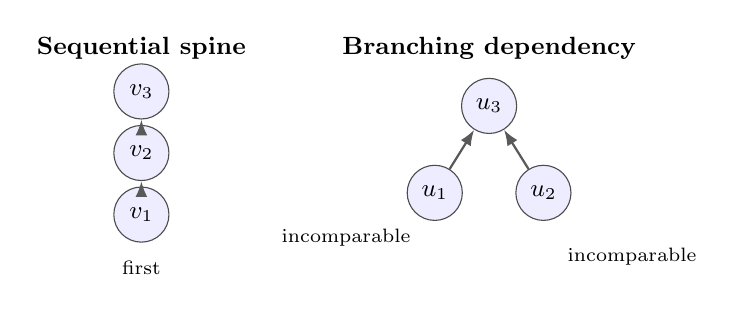
\begin{tikzpicture}[
  scale=0.92,
  every node/.style={font=\small},
  iv/.style={circle,draw=black!70,fill=blue!7,minimum size=7mm,inner sep=0pt},
  dep/.style={-{Latex[length=2mm]},thick,black!65}
]
  \node[font=\small\bfseries] at (-2.4,1.45) {Sequential spine};
  \node[iv] (s3) at (-2.4,0.85) {$v_3$};
  \node[iv] (s2) at (-2.4,0) {$v_2$};
  \node[iv] (s1) at (-2.4,-0.85) {$v_1$};
  \draw[dep] (s1) -- (s2);
  \draw[dep] (s2) -- (s3);
  \node[below=3pt of s1,font=\scriptsize] {first};

  \node[font=\small\bfseries] at (2.4,1.45) {Branching dependency};
  \node[iv] (b3) at (2.4,0.65) {$u_3$};
  \node[iv] (b1) at (1.65,-0.55) {$u_1$};
  \node[iv] (b2) at (3.15,-0.55) {$u_2$};
  \draw[dep] (b1) -- (b3);
  \draw[dep] (b2) -- (b3);
  \node[anchor=north east,font=\scriptsize] at (1.45,-0.92) {incomparable};
  \node[anchor=north west,font=\scriptsize] at (3.35,-1.18) {incomparable};
\end{tikzpicture}
\caption{A sequential tree has a chain of internal dependencies (left).  A
branching tree contains incomparable internal operations and therefore admits
more than one legal internal evaluation order (right).}
\label{fig:sequential-branching-dependency}
\end{figure}

\begin{definition}[Sequential tree]
\label{def:sequential-tree}
A finite binary expression tree satisfying the equivalent conditions of
Theorem~\ref{thm:sequential-tree-classification} is called a
\emph{sequential tree}.
\end{definition}

The adjective refers only to internal evaluation.  It does not choose an
active leaf, and it does not assert that ordinary arithmetic evaluation is
defined.  For example,
\[
  (a+b)(c+d)
\]
is not sequential: the two additions are incomparable dependencies of the
final multiplication.  By contrast,
\[
  \bigl((a+b)c-d\bigr)/e
\]
is sequential, because its internal vertices lie on one spine.

\subsection{One-hole contexts and the marked accumulator}

Let $z$ denote a hole rather than an arithmetic variable.  For
$\omega\in\Omega$ and $c\in K$, define the two elementary one-hole contexts
\begin{equation}
  C_{\omega,c}^{(1)}[z]=\omega(z,c),
  \qquad
  C_{\omega,c}^{(2)}[z]=\omega(c,z).
  \label{eq:elementary-one-hole-contexts}
\end{equation}
The superscript gives the operand slot occupied by the evolving value.  It is
therefore intrinsic to the marked process and should not be replaced by a
description based on how a planar drawing happens to expand.

At the innermost internal vertex of a nontrivial sequential tree, both children
are leaves.  The dependency poset determines that this operation is performed
first, but it does not determine which of its two inputs is the value to be
carried along the spine.  Choosing one of those leaves as the initial
accumulator removes this ambiguity.

\begin{definition}[Marked spinal history]
\label{def:marked-spinal-history}
A \emph{free marked spinal history over $K$} is a finite chronological word
\[
  \gamma=(g_1,\ldots,g_n),
  \qquad
  g_i=C_{\omega_i,c_i}^{(\varepsilon_i)},
  \quad \varepsilon_i\in\{1,2\}.
\]
The context $g_1$ is applied first and $g_n$ last.  Its \emph{chirality word}
is
\[
  \varepsilon(\gamma)=\varepsilon_1\cdots\varepsilon_n.
\]
A \emph{bounded marked spinal history} is a pair $(x_0;\gamma)$ consisting of
an initial accumulator $x_0$ and a free history.  The empty word is allowed;
its bounded form represents the marked single-leaf tree.
\end{definition}

When no confusion is possible, we call either form a marked spinal history and
state explicitly whether an initial value is present.  Earlier drafts called
certain pure-chirality cases threadlike expressions.  The present definition
also includes mixed chirality and makes the marking part of the data.

Figure~\ref{fig:slot-chirality-histories} displays operand-slot chirality
directly in the one-hole contexts.  The diagram is a notation guide, not a
substitute for the marked-tree correspondence proved below.

\begin{figure}[t]
\centering
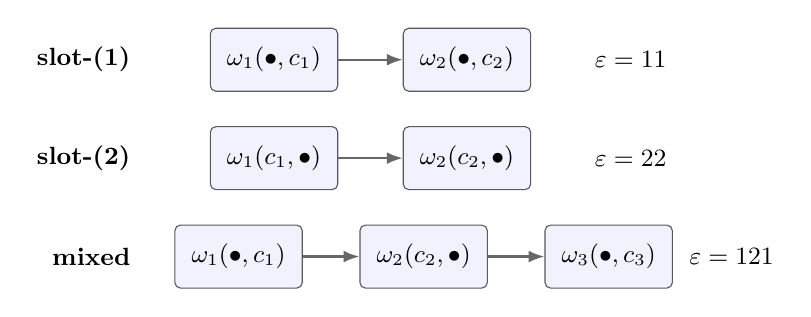
\begin{tikzpicture}[
  box/.style={draw=black!65,rounded corners=2pt,fill=blue!5,
              minimum height=8mm,inner xsep=6pt,font=\small},
  chronarrow/.style={-{Latex[length=2mm]},thick,black!60},
  rowlabel/.style={font=\small\bfseries,anchor=east}
]
  \node[rowlabel] at (-3.6,1.25) {slot-(1)};
  \node[box] (a11) at (-1.9,1.25) {$\omega_1(\bullet,c_1)$};
  \node[box] (a12) at (0.55,1.25) {$\omega_2(\bullet,c_2)$};
  \draw[chronarrow] (a11) -- (a12);
  \node[anchor=west,font=\small] at (2.05,1.25) {$\varepsilon=11$};

  \node[rowlabel] at (-3.6,0) {slot-(2)};
  \node[box] (a21) at (-1.9,0) {$\omega_1(c_1,\bullet)$};
  \node[box] (a22) at (0.55,0) {$\omega_2(c_2,\bullet)$};
  \draw[chronarrow] (a21) -- (a22);
  \node[anchor=west,font=\small] at (2.05,0) {$\varepsilon=22$};

  \node[rowlabel] at (-3.6,-1.25) {mixed};
  \node[box] (am1) at (-2.35,-1.25) {$\omega_1(\bullet,c_1)$};
  \node[box] (am2) at (0,-1.25) {$\omega_2(c_2,\bullet)$};
  \node[box] (am3) at (2.35,-1.25) {$\omega_3(\bullet,c_3)$};
  \draw[chronarrow] (am1) -- (am2);
  \draw[chronarrow] (am2) -- (am3);
  \node[anchor=west,font=\small] at (3.25,-1.25) {$\varepsilon=121$};
\end{tikzpicture}
\caption{Pure slot-(1), pure slot-(2), and mixed marked histories.  In each
box, $\bullet$ is the current accumulator---the marked seed in the first box
and the preceding output thereafter.  Its displayed position is the operand
slot, while time always runs along the arrows.}
\label{fig:slot-chirality-histories}
\end{figure}

\begin{proposition}[Marked-tree--history correspondence]
\label{prop:marked-tree-history-correspondence}
Let $T$ be a sequential tree all of whose leaves are labelled by elements of
$K$.
\begin{enumerate}
  \item If $T$ is a single leaf, marking that leaf determines the empty bounded
  history.
  \item If $T$ is nontrivial, a choice of one leaf at its innermost internal
  vertex as the initial accumulator determines a unique bounded marked spinal
  history.
  \item Conversely, a bounded marked spinal history determines a unique marked
  planar sequential tree.
\end{enumerate}
These two constructions are mutually inverse when operation labels, constants,
operand slots, and the initial mark are retained.
\end{proposition}

\begin{proof}
The single-leaf case is immediate.  Suppose $T$ is nontrivial.  By
Theorem~\ref{thm:sequential-tree-classification}, its internal vertices form a
unique spine.  At the innermost vertex, mark one leaf $x_0$ and denote the
other by $c_1$.  The operation label and the slot containing $x_0$ determine
$g_1=C_{\omega_1,c_1}^{(\varepsilon_1)}$.  Move one vertex towards the root.
Its off-spine child must be a leaf, since otherwise it would be a second
internal child.  Its label $c_2$, the operation label, and the slot occupied by
the spine determine $g_2$.  Repeating this procedure reaches the root and
produces a unique chronological word $(g_1,\ldots,g_n)$.

Conversely, start with a marked leaf $x_0$.  Replace it by the planar binary
tree $C_{\omega_1,c_1}^{(\varepsilon_1)}[x_0]$, then place the resulting tree
in slot $\varepsilon_2$ of the next context, and continue.  Exactly one child
at every new internal vertex is internal, so the result is sequential.  Each
step records the operation, off-spine leaf, and slot used in the forward
construction.  The constructions therefore recover one another.
\end{proof}

The proposition concerns fully labelled planar trees.  If parentheses,
constant labels, or the marked seed are forgotten, the correspondence is no
longer injective.

\subsection{Composition and ordinary evaluation}

If
\[
  \gamma=(g_1,\ldots,g_m),
  \qquad
  \delta=(h_1,\ldots,h_n),
\]
their chronological concatenation is
\begin{equation}
  \gamma\delta=(g_1,\ldots,g_m,h_1,\ldots,h_n),
  \label{eq:chronological-history-concatenation}
\end{equation}
so $\gamma$ is performed first and $\delta$ second.  This convention is fixed
for the entire paper and is summarized again in Appendix~\ref{app:conventions}.

Each elementary context determines a partial function $g_i\colon K\dashrightarrow
K$.  Starting from $x\in K$, define recursively
\[
  x_0=x,
  \qquad
  x_i=g_i(x_{i-1}).
\]
The bounded history is \emph{ordinarily admissible at $x$} when every $x_i$
is defined in ordinary field arithmetic.  In that case its endpoint is
\begin{equation}
  \nu_x(\gamma)
  =g_n\circ\cdots\circ g_1(x).
  \label{eq:ordinary-history-evaluation}
\end{equation}
The admissible domain of a free history is the set of such $x$.  In particular,
a second-slot division $c/z$ excludes any state at which the evolving value is
zero, while a first-slot division $z/c$ requires $c\neq0$.

The concatenation convention gives
\begin{equation}
  \nu_x(\gamma\delta)
  =\nu_{\nu_x(\gamma)}(\delta)
  \label{eq:ordinary-evaluation-concatenation}
\end{equation}
whenever both sides are ordinarily admissible.  Equation
\eqref{eq:ordinary-evaluation-concatenation} is a statement about partial
functions.  Chapter~\ref{sec:projective-affine} introduces a projective
evaluation with a different domain convention.

\subsection{Mirror, temporal reversal, and path inverse}

Three operations on a context word must be kept separate.

\begin{definition}[Mirror and temporal reversal]
\label{def:mirror-temporal-reversal}
For $g=C_{\omega,c}^{(\varepsilon)}$, let
\[
  m(g)=C_{\omega,c}^{(3-\varepsilon)}.
\]
The \emph{mirror} and \emph{temporal reversal} of
$\gamma=(g_1,\ldots,g_n)$ are respectively
\[
  m\gamma=(m(g_1),\ldots,m(g_n)),
  \qquad
  r\gamma=(g_n,\ldots,g_1).
\]
The mirror exchanges operand slots while retaining chronological order;
temporal reversal reverses chronological order while retaining the contexts.
\end{definition}

Both operations are involutions on marked words, and they commute:
$m(r\gamma)=r(m\gamma)$.  This is a syntactic statement; ordinary domains of
the evaluated words need not agree.

\begin{definition}[Path inverse]
\label{def:path-inverse}
Suppose every context $g_i$ in $\gamma$ acts as an invertible function on a
declared domain.  The \emph{path inverse} is the functional word
\[
  \gamma^{-1}=(g_n^{-1},\ldots,g_1^{-1}).
\]
It is defined only under this invertibility hypothesis and need not have the
same operation labels or ordinary admissible domain as $r\gamma$.
\end{definition}

For example, let $g_1[z]=z+1$ and $g_2[z]=2z$.  Then
\[
  \gamma=(g_1,g_2)\colon x\longmapsto2x+2.
\]
Because addition and multiplication are symmetric operations,
$m\gamma$ has the displayed expression $2(1+x)$ and induces the same operator
$2x+2$.  In contrast,
\[
  r\gamma=(g_2,g_1)\colon x\longmapsto2x+1,
\]
while
\[
  \gamma^{-1}=(z\mapsto z/2,\ z\mapsto z-1)
  \colon x\longmapsto x/2-1.
\]
Thus equality with a mirror in this example is caused by the symmetry of the
chosen elementary operations; it does not identify mirror, reversal, and
inverse.  The affine order defect studied later compares temporal orders.  It
is not automatically an invariant of planar mirror.

\subsection{Information retained and information forgotten}

Several equivalence relations occur naturally, and the remainder of the paper
uses them at different stages.  It is useful to order them by the information
they forget.

\begin{enumerate}
  \item \emph{Literal syntactic equality} retains the fully parenthesized
  written expression.
  \item \emph{Marked-history equality} retains the initial mark, the
  chronological context word, and every operand-slot label.  It may forget
  inessential typography but not process data.
  \item \emph{Operator equality} identifies histories inducing the same
  partial function on a stated ordinary domain, or the same projective
  transformation after projective evaluation.
  \item \emph{Charge equality}, when a charge map has been specified, retains
  only the chosen abelian totals of a history.
  \item \emph{Endpoint equality} at $x$ asks only whether the admissible values
  $\nu_x(\gamma)$ and $\nu_x(\delta)$ coincide.
  \item \emph{Quotient or relational equality} is any further identification
  imposed by an explicitly declared rewriting or condensation relation.
\end{enumerate}

This list is not a claim that every adjacent pair gives a strict quotient in
all languages.  It is a discipline for stating which level is being used.
For example, the two histories
\[
  \gamma=(z\mapsto z+1,\ z\mapsto2z),
  \qquad
  \delta=(z\mapsto3z,\ z\mapsto z+1)
\]
are distinct marked histories and induce the distinct operators $2z+2$ and
$3z+1$, but at the initial value $x=1$ both have endpoint $4$.

\subsection{Representative chirality patterns}

The slot notation exposes examples that the older comb terminology obscured.

\begin{example}[Pure slot-(1) history]
The word
\[
  C_{+,2}^{(1)},\quad C_{\times,3}^{(1)},\quad C_{-,4}^{(1)}
\]
has chirality word $111$ and evaluates ordinarily as
$x\mapsto (x+2)3-4$.
\end{example}

\begin{example}[Pure slot-(2) history]
The word
\[
  C_{-,2}^{(2)},\quad C_{/,3}^{(2)}
\]
has chirality word $22$ and evaluates as
\[
  x\longmapsto \frac{3}{2-x},
\]
on the ordinary domain $K\setminus\{2\}$.  The accumulator occupies the
second operand slot at both steps.
\end{example}

\begin{example}[Mixed chirality]
The word
\[
  C_{-,1}^{(1)},\quad C_{/,2}^{(2)},\quad C_{+,3}^{(1)}
\]
has chirality word $121$ and evaluates as
\[
  x\longmapsto \frac{2}{x-1}+3,
\]
on its ordinary domain.  Its dependency poset is still a chain; mixed
chirality does not introduce branching.
\end{example}

The syntactic passage is therefore
\[
  \begin{gathered}
    \text{unmarked sequential tree}
    \xrightarrow{\text{choice of accumulator}}
    \text{marked planar sequential tree},\\
    \text{marked planar sequential tree}
    \longleftrightarrow
    \text{bounded marked spinal history},\\
    \text{bounded marked spinal history}
    \longrightarrow
    \text{operator}
    \longrightarrow
    \text{endpoint}.
  \end{gathered}
\]
when the history is bounded and all planar labels are retained.  The first arrow is a
choice and the double arrow is a bijection; only the later evaluation arrows forget
process data.  Chapter~\ref{sec:projective-affine}
constructs the operator stage for all non-degenerate bilateral contexts.

\subsection{The prefix information order and ideal completion}

The chronological concatenation of \eqref{eq:chronological-history-concatenation}
makes the free marked spinal histories $\Gamma^*$ a monoid.  Domain theory turns
this monoid into an ordered and then a complete object.  Throughout,
$\Gamma=\{\,C_{\omega,c}^{(\varepsilon)}\,\}$ denotes the alphabet of elementary
one-hole contexts.

\begin{definition}[Prefix information order]
\label{def:prefix-information-order}
For free marked spinal histories $\gamma,\gamma'\in\Gamma^*$, write
$\gamma\sqsubseteq\gamma'$ when $\gamma'=\gamma\delta$ for some
$\delta\in\Gamma^*$.  This is the \emph{chronological prefix order}: $\gamma$ is
an earlier truncation of $\gamma'$, retaining strictly less process data.
\end{definition}

The prefix order is a partial order, but $\Gamma^*$ is not directed complete: an
infinite chain $\gamma_0\sqsubseteq\gamma_1\sqsubseteq\cdots$ has no join in
$\Gamma^*$.  Its completion is the classical ideal completion of a poset.

\begin{proposition}[Spinal ideal completion]
\label{prop:spinal-ideal-completion}
The ideal completion of $(\Gamma^*,\sqsubseteq)$ is
\[
\operatorname{Idl}(\Gamma^*)\ \cong\ \Gamma^{\le\omega}:=\Gamma^*\cup\Gamma^\omega,
\]
the dcpo of finite and countably infinite chronological words, ordered by
prefix.  Its compact elements are exactly the finite words $\Gamma^*$, and each
infinite word $\gamma_\infty=(g_1,g_2,\ldots)$ is the directed join of its
finite prefixes:
\[
\gamma_\infty=\bigsqcup_{n\ge0}(g_1,\ldots,g_n).
\]
\end{proposition}

\begin{proof}
The ideals of a prefix-ordered free monoid are exactly the principal ideals
$\mathord\downarrow\gamma$ for finite $\gamma$ and the directed families of all
finite prefixes of an infinite word; the bijection sends an infinite word to the
directed union of its prefixes.  This is the standard ideal-completion
construction for the domain of finite and infinite words
\cite{Scott1972ContinuousLattices,GHKLM2003ContinuousLattices}.
\end{proof}

\subsection{Branching histories and the down-set information order}

The prefix order is the special case in which the dependency poset is a chain.
For a general (branching) tree the internal dependency poset
$P=(I(T),\preccurlyeq_T)$ is not a chain, and the natural information order is
the \emph{down-set} (order-ideal) embedding.

\begin{definition}[Down-set information order]
\label{def:downset-information-order}
Let $\operatorname{FinDAG}$ be the class of finite computation DAGs: finite
dependency posets $P$ whose vertices carry operation, constant, and operand-slot
decorations, as in Definition~\ref{def:internal-dependency-poset}.  For
$P,Q\in\operatorname{FinDAG}$, write $P\sqsubseteq Q$ when $P$ is a decorated
\emph{down-set} (order ideal) of $Q$: $P\subseteq Q$, the order of $P$ is the
restriction of that of $Q$, and
\[
x\in P,\ y\in Q,\ y\le_Q x \ \Longrightarrow\ y\in P .
\]
Read ``$P\sqsubseteq Q$'' as ``$P$ is a completed sub-computation of $Q$''.
\end{definition}

Directed families under $\sqsubseteq$ are towers of sub-computations, and their
direct union is a well-defined (possibly infinite) poset.  The completion is
again classical.

\begin{theorem}[Branching DAG dcpo]
\label{thm:branching-dag-dcpo}
The ideal completion $\operatorname{Idl}(\operatorname{FinDAG},\sqsubseteq)$ is
isomorphic to the class of computation DAGs in which every vertex has only
finitely many predecessors (equivalently, DAGs that are the directed union of
their finite down-sets).  The compact elements are exactly the finite
computation DAGs, and each such infinite DAG $Q$ is the directed join of its
finite down-sets:
\[
Q=\bigsqcup\{\,P\subseteq Q:P \text{ finite down-set}\,\}.
\]
A ``broom'' DAG --- infinitely many minimal vertices feeding a single top
vertex --- is excluded, because its top vertex has infinitely many predecessors
and lies in no finite down-set.  When $P$ is a chain (a sequential tree), the
down-set order restricts to the prefix order of
Definition~\ref{def:prefix-information-order}.
\end{theorem}

\begin{proof}
An ideal $I$ is a directed, downward-closed family of finite DAGs; its direct
union $\bigcup I$ is well-defined, and every element of it lies in some finite
member of $I$ (hence has finitely many predecessors).  Conversely, a DAG in
which every vertex has finitely many predecessors is the direct union of its
finite down-sets, and that family is an ideal.  The two maps are inverse.  The
excluded-broom observation is immediate, and the chain specialization is the
bijection between the down-sets of a chain and its prefixes.
\end{proof}

\subsection{Partial evaluations and Birkhoff duality}

For a fixed finite dependency poset $P$, the partial evaluations --- the
completed sub-computations --- form a finite distributive lattice, and the legal
evaluation orders are its maximal chains.

\begin{theorem}[Down-set lattice and spinal histories]
\label{thm:birkhoff-downset-spinal}
Let $P=I(T)$ be the internal dependency poset of a finite expression tree $T$,
and let $\mathcal{O}(P)$ be its set of down-sets ordered by inclusion.
\begin{enumerate}
  \item $\mathcal{O}(P)$ is a finite distributive lattice --- the lattice of
  partial evaluations of $T$ --- and by Birkhoff duality
  $\operatorname{Stone}(\mathcal{O}(P))\cong P$ (the join-irreducibles recover
  the dependency poset).
  \item The legal internal evaluation orders of $T$ are in bijection with the
  maximal chains
  \[
  \varnothing=D_0\subsetneq D_1\subsetneq\cdots\subsetneq D_{|P|}=P
  \]
  of $\mathcal{O}(P)$, each step adjoining one minimal vertex.
  \item After a choice of initial accumulator and operand-slot marking, each
  maximal chain encodes exactly one marked spinal history.  A sequential tree is
  the case in which $\mathcal{O}(P)$ is a single chain; a branching tree has
  $\mathcal{O}(P)$ a nontrivial distributive lattice, and its complete
  evaluation space is organized by $\mathcal{O}(P)$ together with its maximal
  chains.
\end{enumerate}
\end{theorem}

\begin{proof}
Part (1) is Birkhoff's representation theorem.  For part (2), a maximal chain
from $\varnothing$ to $P$ must add exactly one vertex at a time, and the added
vertex is minimal in the complement, so the sequence of additions is precisely a
linear extension of $P$; the converse is direct.  Part (3) reads that linear
extension through the marked-tree--history correspondence of
Proposition~\ref{prop:marked-tree-history-correspondence}.
\end{proof}

\section{Projective Semantics and the Affine Sector}\label{sec:projective-affine}
% Canonical Paper I source.
The four arithmetic operations behave asymmetrically once the accumulator may
occupy either operand slot.  Most elementary contexts are affine, but the
second-slot division $c/z$ is genuinely projective.  This section makes that
enlargement precise.  The projective semantics does not replace ordinary
arithmetic evaluation: it supplies an operator-valued continuation on a
different domain.

Throughout this section, $K$ is an arbitrary field.  Points of the projective
line are one-dimensional subspaces of $K^2$, written in homogeneous coordinates
as
\[
  [u:v],
  \qquad (u,v)\ne(0,0).
\]
We use the affine chart $z=[z:1]$ and write $\infty=[1:0]$.  Matrices act on
column vectors from the left.  Thus
\begin{equation}
  M=\begin{pmatrix}A&B\\ C&D\end{pmatrix}
  \quad\Longrightarrow\quad
  M\cdot z=\frac{Az+B}{Cz+D},
  \label{eq:column-mobius-action}
\end{equation}
with the homogeneous interpretation at poles and at infinity.  Replacing $M$
by a nonzero scalar multiple does not change the projective map.

\subsection{Ordinary domains and projective continuation}

For an elementary context $g=C_{\omega,c}^{(\varepsilon)}$, ordinary
evaluation gives a partial function $g\colon K\dashrightarrow K$.  A
\emph{non-degenerate projective context} is one for which the corresponding
homogeneous matrix is invertible.  It acts everywhere on $\mathbb P^1(K)$,
although its affine-coordinate formula may have a pole.

The elementary contexts and matrix representatives are as follows.
\begin{center}
\renewcommand{\arraystretch}{1.35}
\begin{tabular}{lll}
\toprule
Context & Affine-coordinate map & Matrix representative \\
\midrule
$C_{+,c}^{(1)}=C_{+,c}^{(2)}$
& $z\mapsto z+c$
& $\begin{pmatrix}1&c\\0&1\end{pmatrix}$ \\
$C_{-,c}^{(1)}$
& $z\mapsto z-c$
& $\begin{pmatrix}1&-c\\0&1\end{pmatrix}$ \\
$C_{-,c}^{(2)}$
& $z\mapsto c-z$
& $\begin{pmatrix}-1&c\\0&1\end{pmatrix}$ \\
$C_{\times,c}^{(1)}=C_{\times,c}^{(2)}$
& $z\mapsto cz$
& $\begin{pmatrix}c&0\\0&1\end{pmatrix}$ \\
$C_{/,c}^{(1)}$
& $z\mapsto z/c$
& $\begin{pmatrix}1&0\\0&c\end{pmatrix}$ \\
$C_{/,c}^{(2)}$
& $z\mapsto c/z$
& $\begin{pmatrix}0&c\\1&0\end{pmatrix}$ \\
\bottomrule
\end{tabular}
\end{center}
The first three rows are invertible for every $c\in K$.  Multiplication by
$c$, first-slot division by $c$, and second-slot division with numerator $c$
are projectively invertible precisely when $c\ne0$.  At $c=0$, multiplication
and $0/z$ are constant on their ordinary domains, while $z/0$ has empty
ordinary domain.  Their singular matrix representatives do not act everywhere
on $\mathbb P^1(K)$: each has a projective base point.  They are therefore
excluded from $\operatorname{PGL}_2(K)$ and from the non-degenerate history
language used below.

The table also displays the distinction between ordinary and projective
domains.  If $c\ne0$, ordinary first-slot division $z/c$ is defined on all of
$K$.  Ordinary second-slot division $c/z$ is defined only for $z\ne0$.
Projectively, the latter sends $0$ to $\infty$ and $\infty$ to $0$.  This is a
valid action on $\mathbb P^1(K)$ but not an ordinary evaluation through a
division by zero.

\begin{warning}[Projective values are not ordinary values]
\label{warn:projective-not-ordinary}
Projective continuation records a fractional linear operator and its chart
transitions.  It does not certify that the original arithmetic word is
ordinarily admissible at a given initial value.  Whenever an endpoint in $K$
is used as an ordinary arithmetic result, ordinary admissibility must be
checked separately.
\end{warning}

\subsection{Projective evaluation of a chronological history}

Let $\operatorname{Hist}^{\mathrm{nd}}_K$ denote the free marked spinal
history language generated by the non-degenerate elementary contexts in the
table.  The superscript ``nd'' refers to projective non-degeneracy, not to
ordinary admissibility at every affine input.

\begin{definition}[Projective evaluation]
\label{def:projective-evaluation}
Choose for each elementary non-degenerate context $g_i$ a matrix representative
$M_i\in\operatorname{GL}_2(K)$.  For the chronological word
$\gamma=(g_1,\ldots,g_n)$, with $g_1$ applied first, define
\begin{equation}
  \rho(\gamma)=[M_n\cdots M_1]
  \in\operatorname{PGL}_2(K).
  \label{eq:projective-evaluation-product}
\end{equation}
For the empty word, set $\rho(\varnothing)=1$.
\end{definition}

This definition uses projective operator evaluation.  For a bounded history
$(x;\gamma)$, its projective endpoint is $\rho(\gamma)\cdot x$ in
$\mathbb P^1(K)$.  Its ordinary endpoint $\nu_x(\gamma)$ remains the partial
evaluation defined in Section~\ref{sec:sequential-histories}.

\begin{proposition}[Compatibility with chronology]
\label{prop:projective-evaluation-chronology}
Projective evaluation is independent of the chosen scalar matrix
representatives.  If $\gamma\delta$ means first $\gamma$ and then $\delta$,
then
\begin{equation}
  \rho(\gamma\delta)=\rho(\delta)\rho(\gamma).
  \label{eq:rho-chronological-antihomomorphism}
\end{equation}
Moreover, whenever $\gamma$ is ordinarily admissible at $x$ and its ordinary
endpoint lies in $K$, the projective endpoint agrees with it in the affine
chart:
\[
  \rho(\gamma)\cdot x=[\nu_x(\gamma):1].
\]
\end{proposition}

\begin{proof}
Replacing $M_i$ by $a_iM_i$, with $a_i\in K^\times$, multiplies the product
$M_n\cdots M_1$ by the nonzero scalar $\prod_i a_i$ and hence does not alter
its projective class.  If
$\gamma=(g_1,\ldots,g_m)$ and $\delta=(h_1,\ldots,h_n)$, then the matrix word
for $\gamma\delta$ is
\[
  N_n\cdots N_1M_m\cdots M_1,
\]
which represents $\rho(\delta)\rho(\gamma)$.  This proves
\eqref{eq:rho-chronological-antihomomorphism}.

For the last assertion, each row of the table agrees with its ordinary
arithmetic context wherever that context is defined.  Applying this observation
inductively along the admissible intermediate states proves equality in the
affine chart.
\end{proof}

Thus $\rho$ is a homomorphism from chronological words if the target group is
written with the opposite multiplication.  We retain ordinary matrix
multiplication and the explicit rule
\eqref{eq:rho-chronological-antihomomorphism}, because it makes both the column
action and function composition standard.

\subsection{Generation of the projective group}

Introduce the elementary projective transformations
\[
  T_s(z)=z+s,
  \qquad
  D_q(z)=qz\quad(q\in K^\times),
  \qquad
  J(z)=-\frac1z.
\]
They are projective evaluations of, respectively, addition by $s$,
multiplication by $q$, and second-slot division with numerator $-1$.  These
three kinds of context suffice for the entire bilateral projective language at
the operator level.

\begin{theorem}[Bilateral arithmetic generates $\operatorname{PGL}_2$]
\label{thm:bilateral-pgl2-generation}
Let $K$ be any field.  The projective evaluations of non-degenerate bilateral
four-operation marked spinal histories have image
\[
  \rho\bigl(\operatorname{Hist}^{\mathrm{nd}}_K\bigr)
  =\operatorname{PGL}_2(K).
\]
Equivalently, translations $T_s$, nonzero
scalings $D_q$, and $J$ generate $\operatorname{PGL}_2(K)$.
\end{theorem}

\begin{proof}
The inclusion $\rho(\operatorname{Hist}^{\mathrm{nd}}_K)\subseteq
\operatorname{PGL}_2(K)$ holds by definition: every elementary context admitted
to $\operatorname{Hist}^{\mathrm{nd}}_K$ has an invertible matrix
representative, and a product of invertible matrices is invertible.

% Cross-paper reference: Paper 0 label thm:p0-pgl2-generation; it is
% Theorem 6.2 of Paper 0 in the 2026-10-29 build.  If that numbering changes,
% update this citation and the one in Subsection 3.7.
For the converse, each of $T_s$, $D_q$, and $J$ is an elementary non-degenerate
context of the table above, so the image contains the subgroup they generate.
That subgroup is all of $\operatorname{PGL}_2(K)$ by the generation theorem for
projective arithmetic, which is Theorem~6.2 of Paper~0 and is proved there for
an arbitrary field without any ordering or characteristic hypothesis.  Reading
that theorem through the present history language gives the stated equality.
\end{proof}

The generation statement is therefore a theorem of the series rather than of
this paper alone: its proof, and the constructive factorization it yields, are
in Paper~0.  What belongs to this paper is the reading of that factorization as
a chronological word.  Paper~0's proof is constructive, giving a history of
length at most four for any specified projective matrix once arbitrary field
constants are admitted as context parameters.  It establishes surjectivity at
the operator level, not uniqueness of a representing history.  In fact, many
distinct context words have the same projective evaluation.

\begin{example}[A pole in an ordinarily inadmissible history]
Let $K=\mathbb Q$ and consider the one-step history $g[z]=1/z$.  It is a
non-degenerate projective context with $\rho(g)\cdot0=\infty$.  The bounded
history $(0;g)$ has no ordinary endpoint.  Appending another inversion gives a
projective word acting as the identity, but the two-step ordinary evaluation
at $0$ is still inadmissible because its first step is undefined.
\end{example}

\subsection{A distinguished arithmetic sublanguage: the q=4 Hecke group}
\label{subsec:hecke-four-interface}

The surjectivity theorem allows arbitrary constants and produces the whole
projective group.  A much smaller constant alphabet already carries a useful
discrete geometry.  Work in
\(\mathbb Q(\sqrt2)\subset\mathbb R\), and let
\(\operatorname{Hist}_4\) be the symmetric marked history language generated
by the three elementary contexts
\[
  \mathsf t_+[z]=z+\sqrt2,
  \qquad
  \mathsf t_-[z]=z-\sqrt2,
  \qquad
  \mathsf j[z]=-\frac1z.
\]
Here ``symmetric'' means that the inverse translation is retained as a
generator; \(\mathsf j\) is its own projective inverse.  Write
\[
  T=T_{\sqrt2},
  \qquad
  G_4=\rho(\operatorname{Hist}_4)
      =\langle T,J\rangle
      \leq \operatorname{PGL}_2(\mathbb R).
\]
This is the standard projective realization of the $q=4$ Hecke group
\cite{Rosen1954ContinuedFractions,LangLang2016HeckeGroups}.

\begin{proposition}[The order-four arithmetic relation]
\label{prop:hecke-four-arithmetic-relation}
With the column action and chronological convention fixed above, the generators
have determinant-one representatives
\[
  \widetilde T=
  \begin{pmatrix}1&\sqrt2\\0&1\end{pmatrix},
  \qquad
  \widetilde J=
  \begin{pmatrix}0&-1\\1&0\end{pmatrix}
  \quad\text{in }\operatorname{SL}_2(\mathbb Z[\sqrt2]).
\]
Consequently $G_4$ is defined by matrices over $\mathbb Z[\sqrt2]$.  In
$\operatorname{PGL}_2(\mathbb R)$ one has
\begin{equation}
  J^2=1,
  \qquad
  (JT)^4=1,
  \label{eq:hecke-four-relations}
\end{equation}
and $JT$ has exact projective order four.  The second relation is the
projective evaluation of the chronological eight-step history
\begin{equation}
  \omega_4=(\mathsf t_+,\mathsf j,
             \mathsf t_+,\mathsf j,
             \mathsf t_+,\mathsf j,
             \mathsf t_+,\mathsf j).
  \label{eq:hecke-four-history}
\end{equation}
Thus $\omega_4$ and the empty history are distinct marked histories with the
same projective operator.
\end{proposition}

\begin{proof}
Both displayed matrices have determinant one and entries in
$\mathbb Z[\sqrt2]$; their inverses have the same property.  Moreover,
\[
  \widetilde J^2=-I,
  \qquad
  R:=\widetilde J\widetilde T
    =\begin{pmatrix}0&-1\\1&\sqrt2\end{pmatrix},
  \qquad
  R^2=\begin{pmatrix}-1&-\sqrt2\\
                       \sqrt2&1\end{pmatrix}.
\]
A second multiplication gives $R^4=-I$.  Hence the scalar classes satisfy
\eqref{eq:hecke-four-relations}.  Neither $R$ nor $R^2$ is scalar, so the
projective order of $JT$ is exactly four.  Finally, each chronological pair
$(\mathsf t_+,\mathsf j)$ evaluates as $J\circ T$ and is represented by
$\widetilde J\widetilde T=R$.  Four such pairs therefore evaluate as $R^4$,
which is the identity in the projective group.
\end{proof}

The proposition is an operator statement, not a universal statement about
ordinary real arithmetic.  Every letter of $\operatorname{Hist}_4$ is
projectively non-degenerate, but a bounded history is ordinarily admissible
only if the evolving affine value is nonzero whenever $\mathsf j$ is applied.
For example, $\omega_4$ is projectively neutral but is not ordinarily
admissible at $x=-\sqrt2$: its first translation reaches zero, after which
$\mathsf j$ requests division by zero.  In contrast, the same matrices act
without an interior pole on the upper half-plane $\mathbb H^2$.  The Fuchsian
action and ordinary evaluation on a specified real input are therefore two
related but distinct uses of the same context word.

\begin{remark}[From histories to Hecke cells]
\label{rem:hecke-history-operator-coset}
The conventional action of $G_4$ on $\mathbb H^2$ supplies its Hecke
tessellations and derived dual cellulations.  Paper~I needs only the following
formal interface.  If $\mathcal C$ is a chosen cell in such a
$G_4$-equivariant cellulation and
\(H_{\mathcal C}=\operatorname{Stab}_{G_4}(\mathcal C)\), then the cell reached
by a history factors as
\begin{equation}
  \operatorname{Hist}_4
    \xrightarrow{\ \rho\ }G_4
    \longrightarrow G_4/H_{\mathcal C},
  \qquad
  \gamma\longmapsto\rho(\gamma)H_{\mathcal C}.
  \label{eq:hecke-history-coset-interface}
\end{equation}
Neither arrow is generally injective.  Relations such as
\eqref{eq:hecke-four-history} identify distinct histories at the operator
level, and distinct operators in one coset act on $\mathcal C$ as the same
cell.  Passing instead to one endpoint uses the stabilizer of that
point and forgets still more information.  Thus arithmetic histories,
projective operators, cells, and endpoints must not be placed in one-to-one
correspondence.  The order-four relation provides an arithmetic entry point
for the fourfold incidence visible in the $q=4$ geometry; the construction of
analytic functions and singular zero sets on that cellulation is deferred to
Papers~II and~III.
\end{remark}

\subsection{The affine syntactic sector}

Let $B_\infty$ be the stabilizer of the chosen point at infinity:
\[
  B_\infty
  =\operatorname{Stab}_{\operatorname{PGL}_2(K)}(\infty).
\]
An element represented by $\begin{pmatrix}A&B\\C&D\end{pmatrix}$ fixes
$\infty=[1:0]$ exactly when $C=0$.  After rescaling by $D^{-1}$, it then has a
unique representative
\[
  \begin{pmatrix}a&b\\0&1\end{pmatrix},
  \qquad a\in K^\times,\quad b\in K,
\]
acting as $z\mapsto az+b$.

Define $\operatorname{Hist}^{\mathrm{aff}}_K$ to be the syntactic sublanguage
generated by those \emph{elementary non-degenerate contexts} in the table that
individually fix $\infty$.  Equivalently, it excludes the elementary
second-slot divisions $c/z$ and retains every non-degenerate elementary affine
context.  This definition is deliberately syntactic: it does not assert that
$\operatorname{Hist}^{\mathrm{aff}}_K$ is the entire inverse image
$\rho^{-1}(B_\infty)$.  A word containing projective steps can leave the
affine chart and later evaluate to an affine operator.

\begin{corollary}[Affine/Borel sector]
\label{cor:affine-borel-sector}
For every field $K$,
\[
  \rho\bigl(\operatorname{Hist}^{\mathrm{aff}}_K\bigr)=B_\infty
  \cong\operatorname{Aff}(1,K).
\]
In particular, the affine syntactic sublanguage maps surjectively onto the
Borel subgroup stabilizing $\infty$.
\end{corollary}

\begin{proof}
Every generator of $\operatorname{Hist}^{\mathrm{aff}}_K$ fixes $\infty$;
therefore every product of their projective matrices fixes $\infty$, and the
image is contained in $B_\infty$.  Conversely, every element of $B_\infty$
acts as $z\mapsto az+b$ with $a\ne0$.  It is
\[
  T_b\circ D_a,
\]
the evaluation of a chronological word consisting of the non-degenerate
affine contexts $D_a$ followed by $T_b$.  Hence the image is all of
$B_\infty$.  The displayed normal form also identifies its group law with
that of $\operatorname{Aff}(1,K)$.
\end{proof}

Figure~\ref{fig:affine-sector-inside-projective} records the resulting
operator-level placement.  It does not identify the affine syntactic language
with the full inverse image of the inner region.

\begin{figure}[t]
\centering
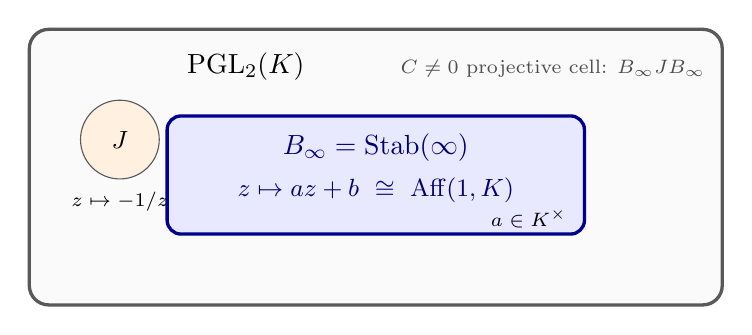
\begin{tikzpicture}[every node/.style={font=\small}]
  \draw[rounded corners=7pt,very thick,draw=black!65,fill=gray!4]
    (-4.4,-1.75) rectangle (4.4,1.75);
  \node[font=\bfseries] at (-1.65,1.28) {$\operatorname{PGL}_2(K)$};
  \node[text=black!70,font=\scriptsize] at (2.25,1.25)
    {$C\ne0$ projective cell: $B_\infty J B_\infty$};
  \node[draw=black!65,circle,fill=orange!12,minimum size=10mm]
    (j) at (-3.25,0.35) {$J$};
  \node[below=1pt of j,font=\scriptsize] {$z\mapsto-1/z$};

  \draw[rounded corners=5pt,very thick,draw=blue!55!black,fill=blue!9]
    (-2.65,-0.85) rectangle (2.65,0.65);
  \node[font=\bfseries,blue!45!black] at (0,0.25)
    {$B_\infty=\operatorname{Stab}(\infty)$};
  \node[blue!45!black] at (0,-0.3)
    {$z\mapsto az+b\ \cong\ \operatorname{Aff}(1,K)$};
  \node[font=\scriptsize,anchor=east] at (2.55,-0.65)
    {$a\in K^\times$};
\end{tikzpicture}
\caption{The affine/Borel sector inside the bilateral projective operator
semantics.  Elementary affine contexts generate the stabilizer $B_\infty$,
whereas inversion reaches the complementary Bruhat cell.  Words containing
projective steps may nevertheless evaluate back into $B_\infty$.}
\label{fig:affine-sector-inside-projective}
\end{figure}

The corollary locates the existing add--multiply language without collapsing
the larger syntax.  Pure slot-(1) non-degenerate histories lie in this affine
sector, but so do second-slot subtraction and multiplication contexts.  The
criterion is stabilization of $\infty$, not the slot bit by itself.

\subsection{The positive real component}

Later differential-geometric sections use real multiplication in the form
\[
  z\longmapsto e^M z,
  \qquad M\in\mathbb R.
\]
Its multiplier is positive.  Together with all real translations, these maps
form
\[
  \operatorname{Aff}^+(1,\mathbb R)
  =\{z\mapsto az+b:a>0\},
\]
the identity component of the real affine group.  They do not include affine
reflections with negative multiplier.  The algebraic statement of
Corollary~\ref{cor:affine-borel-sector} concerns all nonzero multipliers in
$K^\times$; the continuous theory is its positive real component.

\subsection{Bruhat placement and the projective infinitesimal direction}

% Cross-paper reference: see the note in Subsection 3.3.
The case division in the proof of Paper~0, Theorem~6.2 also gives the rank-one
Bruhat decomposition
\[
  \operatorname{PGL}_2(K)=B_\infty\sqcup B_\infty J B_\infty ,
\]
which Paper~0 records in the same chapter.  The first cell is the case
$C=0$; the explicit factorization obtained for $C\ne0$ lies in the second.  The
same dichotomy separates the contexts of the table above: the affine rows fix
$\infty$, and the second-slot division $c/z$ is the elementary step that leaves
the first cell.  This observation places bilateral arithmetic as a projective
completion of the affine sector; no representation-theoretic conclusions beyond
this decomposition are needed here.

There is also an infinitesimal counterpart over $\mathbb R$ (or $\mathbb C$).
The projective vector fields
\[
  \partial_z,
  \qquad z\partial_z,
  \qquad z^2\partial_z
\]
span the local projective Lie algebra.  The first two generate affine flow.  A
conjugated translation detects the third direction:
\[
  J\circ T_s\circ J^{-1}(z)
  =\frac{z}{1-sz}
  =z+sz^2+O(s^2).
\]
Consequently a general scalar projective flow has Riccati form
\[
  \dot z=\beta+\alpha z+\kappa z^2.
\]
Paper~I develops only the affine slice $\kappa=0$.  No projective metric,
projective arithmetic expression space, or projective contact theory is
asserted here.

\section{Analytical Pillar I: Differential Theory}\label{sec:differential-theory}
% Canonical Paper I source.

The differential pillar turns the discrete histories of
Section~\ref{sec:sequential-histories} into continuous flows and identifies the
order defect of the minimal branching DAG with the contact curvature imported
from Paper~0.  Throughout this section $\mu,\lambda$ are the fixed real
intensities of the regular AES of Section~\ref{sec:regular-aes-interface}.

\subsection{The smoothing Lie functor}

Recall the arithmetic contact model $\mathcal C=\mathbb R^3_{(u,v,a)}$ with
contact one-form
\[
  \alpha=da-\mu\,du-\lambda a\,dv,
\]
horizontal fields
\[
  D_u=\partial_u+\mu\,\partial_a,
  \qquad
  D_v=\partial_v+\lambda a\,\partial_a,
\]
and curvature bracket
\[
  [D_u,D_v]=\mu\lambda\,\partial_a
\]
($\texttt{eq:arithmetic-contact-form}$,
$\texttt{eq:horizontal-arithmetic-fields}$,
$\texttt{thm:contact-curvature}$ of Paper~0).  The additive and multiplicative
generators of Section~\ref{sec:sequential-histories} are the exact closed-form
flows of these two fields.

\begin{lemma}[Generators are exact flows]
\label{lem:generators-exact-flows}
The additive generator $A_h=T_{\mu h}$ and the positive multiplicative generator
$M_k=D_{e^{\lambda k}}$ are the time-$h$ and time-$k$ flows of $D_u$ and $D_v$
acting on the assignment fiber:
\[
  A_h(a)=\bigl.\Phi_u^h(0,0,a)\bigr|_a=a+\mu h,
  \qquad
  M_k(a)=\bigl.\Phi_v^k(0,0,a)\bigr|_a=e^{\lambda k}a,
\]
where
\[
  \Phi_u^h(u,v,a)=(u+h,v,a+\mu h),
  \qquad
  \Phi_v^k(u,v,a)=(u,v+k,e^{\lambda k}a).
\]
\end{lemma}

\begin{proof}
Direct substitution: the one-parameter groups of $D_u$ and $D_v$ are the
displayed affine maps, read on the $a$-coordinate.
\end{proof}

\begin{lemma}[Word-to-flow anti-homomorphism]
\label{lem:word-flow-antihomomorphism}
The assignment $F$ sending $A_h\mapsto\Phi_u^h$ and $M_k\mapsto\Phi_v^k$, and a
chronological word to the composition of the corresponding flows, satisfies
\[
  F(\gamma\delta)=F(\delta)\circ F(\gamma),
\]
the same anti-homomorphism as the projective evaluation of
Equation~\eqref{eq:rho-chronological-antihomomorphism}.
\end{lemma}

\begin{proof}
Immediate from the definition on generators and the free-monoid extension.
\end{proof}

\subsection{Minimal DAG defects and contact curvature}

The smallest nontrivial branching history is the two-element antichain
$\{A,M\}$: addition and multiplication are incomparable operations.  Its
evaluation defect is exactly the contact curvature.

\begin{theorem}[DAG defect equals contact curvature]
\label{thm:dag-defect-equals-curvature}
Let $P=\{A,M\}$ be the two-element antichain (addition and multiplication
incomparable).  Its down-set lattice
$\mathcal O(P)=B_2=\{\varnothing,\{A\},\{M\},\{A,M\}\}$ is the four-element free
distributive diamond, with Stone spectrum
$\operatorname{Stone}(\mathcal O(P))=\{A,M\}$, and its two maximal chains are the
two spinal histories $\gamma_1=(A_h,M_k)$ and $\gamma_2=(M_k,A_h)$.
\begin{enumerate}
  \item \textbf{Open and closed defects.} The open order defect is
  \[
    \nu_a(\gamma_1)-\nu_a(\gamma_2)=T_{\mathrm{open}}(h,k)=\mu h(e^{\lambda k}-1),
  \]
  and the four-step closed loop $(A_h,M_k,A_{-h},M_{-k})$ has vertical drift
  \[
    T_{\mathrm{closed}}(h,k)=\mu h(1-e^{-\lambda k})=e^{-\lambda k}T_{\mathrm{open}}(h,k).
  \]
  \item \textbf{Infinitesimal density equals the Lie bracket.}
  \[
    \left.\frac{\partial^2 T_{\mathrm{open}}}{\partial h\,\partial k}\right|_{0,0}
    =
    \left.\frac{\partial^2 T_{\mathrm{closed}}}{\partial h\,\partial k}\right|_{0,0}
    =[D_u,D_v](a)=\mu\lambda .
  \]
  \item \textbf{Structural refinement.} The combinatorial diamond
  $\mathcal O(\{A,M\})$ and its Stone spectrum are flat (curvature zero); the
  curvature $\mu\lambda$ arises at the single step that lifts two directions,
  which commute at the charge level, to a non-commutative realization in the
  value space --- the difference between the semi-direct rescaling law
  $D_k\circ T_s=T_{ks}\circ D_k$ and the naive swap $T_s\circ D_k$.
\end{enumerate}
\end{theorem}

\begin{proof}
(1) is the direct computation
$\nu_a(A_h,M_k)=e^{\lambda k}(a+\mu h)$ versus
$\nu_a(M_k,A_h)=e^{\lambda k}a+\mu h$, and the four-step substitution of
Paper~0 ($\texttt{eq:exact-open-contact-defect}$,
$\texttt{eq:exact-closed-contact-drift}$).  (2) Differentiate:
$\partial^2_h\partial^2_k\,\mu h(e^{\lambda k}-1)\to\mu\lambda$ and
$\partial^2_h\partial^2_k\,\mu h(1-e^{-\lambda k})\to\mu\lambda$, which is
$[D_u,D_v](a)=\mu\lambda\,\partial_a(a)=\mu\lambda$ by
$\texttt{thm:contact-curvature}$.  (3) is the structural reading
$D_k\circ T_s(a)=ka+ks=T_{ks}\circ D_k(a)$ versus $T_s\circ D_k(a)=ka+s$, whose
difference is $s(k-1)=\mu h(e^{\lambda k}-1)$.
\end{proof}

\subsection{Graded horizontal calculus}

The horizontal differential of Paper~0 extends to a graded covariant
differential with a twisted Leibniz law.  Recall the scalar horizontal
differential
\[
  \delta_H F=dF-(\partial_a F)\alpha=(D_uF)\,du+(D_vF)\,dv,
\]
and the curvature operator on scalar fields
\[
  \mathcal R_H(F)=(D_uD_vF-D_vD_uF)\,du\wedge dv=\mu\lambda\,(\partial_aF)\,du\wedge dv
\]
($\texttt{eq:scalar-horizontal-differential}$,
$\texttt{prop:horizontal-differential-curvature}$ of Paper~0).  In the natural
arithmetic units $dA=\mu\,du$, $dM=\lambda\,dv$:

\begin{definition}[Graded horizontal differential]
\label{def:graded-horizontal-differential}
For a smooth section $f$ of integer weight $n\in\mathbb Z$, define the
\emph{weight-$n$ horizontal covariant differential}
\[
  \nabla^{(n)}f:=\delta_H f-n\,f\,dM .
\]
\end{definition}

\begin{proposition}[Graded Leibniz law and gauge rectification]
\label{prop:graded-leibniz-and-gauge}
\begin{enumerate}
  \item The assignment $a$ has weight $1$ and satisfies the propagation law
  \[
    \nabla^{(1)}a=\delta_H a-a\,dM=dA .
  \]
  \item \textbf{Graded Leibniz law.} For $f$ of weight $m$ and $g$ of weight
  $n$,
  \[
    \nabla^{(m+n)}(fg)=\bigl(\nabla^{(m)}f\bigr)\,g+f\,\bigl(\nabla^{(n)}g\bigr).
  \]
  \item \textbf{Gauge rectification and twisted derivative.} Let
  $\widetilde a:=e^{-M}a$ (weight $0$); then
  $\delta_H\widetilde a=e^{-M}dA$.  On a one-parameter curve, define the
  twisted product $(F\star_M G)(t):=e^{-M(t)}F(t)G(t)$ and the twisted
  derivative $D_M:=\frac{d}{dt}-M'(t)=e^{M}\circ\frac d{dt}\circ e^{-M}$; then
  $D_M$ is a strict derivation for $\star_M$:
  \[
    D_M(F\star_M G)=(D_MF)\star_M G+F\star_M(D_M G).
  \]
\end{enumerate}
\end{proposition}

\begin{proof}
(1) $\delta_H a=\mu\,du+\lambda a\,dv$ along horizontal directions, so
$\nabla^{(1)}a=\mu\,du+\lambda a\,dv-a\,\lambda\,dv=\mu\,du=dA$.  (2) Since
$\delta_H$ is a derivation on scalars,
$\delta_H(fg)=(\delta_H f)g+f(\delta_H g)$, whence
$\nabla^{(m+n)}(fg)=(\delta_H f-m f\,dM)g+f(\delta_H g-n g\,dM)$ as claimed.
(3) $\delta_H\widetilde a=e^{-M}(\delta_H a-a\,dM)=e^{-M}dA$; and the
conjugation $D_M=e^{M}\circ\frac d{dt}\circ e^{-M}$ is a derivation for the
multiplicative structure induced by $\star_M$, checked directly.
\end{proof}

\section{Analytical Pillar II: Integral Theory}\label{sec:integral-theory}
% Canonical Paper I source.

The integral pillar has two layers.  In one dimension it is the mixed
additive--multiplicative integral whose two sides are Scott-continuous in the
two directions of Section~\ref{sec:projective-affine}; in higher dimension it is
the order defect as a group-valued $1$-cocycle on the linear-extension graph,
closed by the holographic Stokes theorem.  Throughout, $u,v$ are densities on
$[a,b]$ and $M(t)=\int_a^t v$ is the multiplicative charge.

\subsection{The one-dimensional mixed affine integral}

\begin{definition}[Mixed affine integral]
\label{def:mixed-affine-integral}
For $u,v\in L^1([a,b])$, define the \emph{continuous mixed additive--multiplicative
integral} in absolute-time parametrization,
\[
  \mathfrak M_a^b[u;v]:=\int_a^b u(x)\,\exp\!\Bigl(\int_x^b v(s)\,ds\Bigr)\,dx ,
\]
and, in the right-endpoint sliding-window parametrization, the one-sided
Volterra convolution
\[
  \mathfrak A(w):=\int_0^w u(x)\,K(w-x)\,dx,
  \qquad
  K(r)=\exp\!\Bigl(\int_0^r v(y)\,dy\Bigr).
\]
\end{definition}

\begin{proposition}[Mixed-integral equivalences]
\label{prop:mixed-integral-equivalences}
\begin{enumerate}
  \item \textbf{Affine transport and splitting.} $\mathfrak M_a^b[u;v]$ is the
  inhomogeneous propagation term of the affine transport equation
  $w'(t)=v(t)w(t)+u(t)$:
  \[
    w(b)=e^{\int_a^b v}w(a)+\mathfrak M_a^b[u;v],
  \]
  and satisfies the splitting law and the right-endpoint derivative
  \[
    \mathfrak M_a^c[u;v]=e^{\int_b^c v}\mathfrak M_a^b[u;v]+\mathfrak M_b^c[u;v],
    \qquad
    \frac{d}{db}\mathfrak M_a^b[u;v]=u(b)+v(b)\,\mathfrak M_a^b[u;v].
  \]
  \item \textbf{Window derivative and integration by parts.} For
  $u\in C^1([0,w])$, $v\in C([0,w])$,
  \[
    \mathfrak A'(w)=u(0)K(w)+\int_0^w u'(x)K(w-x)\,dx
    =u(w)+\int_0^w u(x)\,v(w-x)K(w-x)\,dx .
  \]
  \item \textbf{Reverse ACS line integral.} On the accumulative commutative space
  $\mathcal A=\mathbb R^2_{(A,M)}$,
  \[
    \mathfrak M_a^b[u;v]=\int_{C^{\mathrm{rev}}}\eta ,
    \qquad
    \eta=e^M dA ,
  \]
  where $C^{\mathrm{rev}}$ is the ACS path generated by the reversed density.
  \item \textbf{Twisted Rota--Baxter identity.} With
  $(I_M f)(t)=e^{M(t)}\int_{t_0}^t e^{-M(s)}f(s)\,ds=(e^M\circ J\circ e^{-M})f$
  and the twisted product $\star_M$ of
  Proposition~\ref{prop:graded-leibniz-and-gauge},
  \[
    I_M(f)\star_M I_M(g)=I_M\bigl(I_M(f)\star_M g+f\star_M I_M(g)\bigr).
  \]
\end{enumerate}
\end{proposition}

\begin{proof}
(1) Differentiate $e^{-\int_a^t v}w(t)$ to isolate the inhomogeneous term; the
splitting law is the semigroup property of the fundamental solution, and the
endpoint derivative is the transport equation itself.  (2) Differentiate the
convolution under the sign and integrate by parts.  (3) Substitute $A,M$ and
observe that the density $\eta=e^M dA$ integrates along the reversed path to the
displayed form.  (4) is a direct computation using the twisted derivation law
of Proposition~\ref{prop:graded-leibniz-and-gauge}.
\end{proof}

\subsection{Dual adjoint pairing and the Lawson two-sided functional}

The two directions of the mixed integral are not symmetric: the additive source
is the Scott (from-below) side and the multiplicative density is the lower
(dual) side.  Their pairing is the functional form of the Lawson topology.

\begin{theorem}[Lawson dual adjoint pairing]
\label{thm:lawson-dual-adjoint-pairing}
\begin{enumerate}
  \item \textbf{Dual connection.} On the weight-${(-1)}$ dual line, define
  $\nabla^{(-1)}p:=\delta_H p+p\,dM$.  Then
  \[
    \delta_H(pa)=\bigl(\nabla^{(-1)}p\bigr)a+p\,\bigl(\nabla^{(1)}a\bigr),
  \]
  and when $p$ satisfies the homogeneous backward-parallel equation
  $\nabla^{(-1)}p=0$, i.e.\ $-p'(t)=v(t)p(t)$ with $p(b)=1$, one has
  $\delta_H(pa)=p\,dA$, so that
  \[
    \mathfrak M_a^b[u;v]=\int_a^b p(t)\,u(t)\,dt .
  \]
  \item \textbf{Backward adjoint equals the reciprocal image.} With the forward
  scale $K(t)=e^{M(t)}$ and the backward adjoint
  $p(t)=\exp\!\bigl(\int_t^b v(s)\,ds\bigr)$,
  \[
    p(t)=e^{M(b)-M(t)}=K(b)\cdot\neg\bigl(K(t)\bigr),
    \qquad
    \neg(a)=\frac1a .
  \]
  \item \textbf{Bilateral Scott continuity.} For nonnegative densities
  $u,v\ge0$, the functional $u\mapsto\mathfrak M[u;v]$ and
  $v\mapsto\mathfrak M[u;v]$ are each monotone and preserve directed suprema,
  hence are separately Scott-continuous; the pairing $\int_a^b u\,p$ is the
  functional-level realization of the Lawson topology
  $\lambda=\sigma\vee\neg_*\sigma$ of
  Proposition~\ref{prop:generator-domain-roles}.
\end{enumerate}
\end{theorem}

\begin{proof}
(1) is the graded Leibniz law of
Proposition~\ref{prop:graded-leibniz-and-gauge} at weights $-1,1$; solving
$\nabla^{(-1)}p=0$ gives $p(t)=e^{M(b)-M(t)}$.  (2) is the displayed
computation.  (3) monotone convergence gives the directed-sup preservation in
each argument; the forward scale $K$ and the backward adjoint $p=\neg(K)$ carry
the Scott and the lower side respectively.
\end{proof}

\subsection{The order defect as a group-valued $1$-cocycle}

For a general dependency poset $P$ the order defect between two linear
extensions is additive along adjacent swaps, and closed by the Jacobi identity.

\begin{theorem}[Defect group $1$-cocycle]
\label{thm:defect-group-1-cocycle}
Let $P$ be a finite dependency poset and $G(P)$ its linear-extension graph
(vertices are linear extensions $\gamma$, edges are adjacent transpositions of
incomparable elements).
\begin{enumerate}
  \item \textbf{Exact telescoping.} For a path
  $\gamma_0\to\gamma_1\to\cdots\to\gamma_m$ in $G(P)$,
  \[
    \rho(\gamma_m)\rho(\gamma_0)^{-1}
    =\delta(\gamma_{m-1}\to\gamma_m)\cdots\delta(\gamma_0\to\gamma_1),
    \qquad
    \delta(\gamma\to\gamma'):=\rho(\gamma')\rho(\gamma)^{-1},
  \]
  and the scalar defect $\nu_a(\gamma_0)-\nu_a(\gamma_m)$ is the corresponding
  telescoping sum.  Both depend only on the endpoints.
  \item \textbf{Suffix-conjugated commutator.} In a history $\gamma=UxyW$ ($U$
  executed first, $W$ last), swapping adjacent incomparable $x,y$ to
  $\gamma'=UyxW$ gives
  \[
    \delta(UxyW\to UyxW)=\rho(W)\,\bigl[\rho(x),\rho(y)\bigr]\,\rho(W)^{-1},
    \qquad
    [g,h]:=ghg^{-1}h^{-1} .
  \]
  \item \textbf{BCH expansion and Jacobi closure.} With infinitesimal
  generators $e^{hX},e^{kY},e^{lZ}$,
  \[
    [e^{hX},e^{kY}]
    =\exp\Bigl(hk[X,Y]+\tfrac{h^2k}{2}[X,[X,Y]]+\tfrac{hk^2}{2}[Y,[X,Y]]+\cdots\Bigr),
  \]
  and the two three-step paths around the hexagon of a three-element antichain
  $\{X,Y,Z\}$ differ, to third order, by exactly the Jacobi identity
  $[X,[Y,Z]]+[Y,[Z,X]]+[Z,[X,Y]]=0$ (the discrete Bianchi identity
  $d\Omega=0$).
\end{enumerate}
\end{theorem}

\begin{proof}
(1) is the telescoping product; (2) is the direct computation
$\rho(UyxW)\rho(UxyW)^{-1}=\rho(W)\rho(x)\rho(y)\rho(x)^{-1}\rho(y)^{-1}\rho(W)^{-1}$;
(3) is the Campbell--Baker--Hausdorff formula and the vanishing of its
third-order mixed term by the Jacobi identity.
\end{proof}

\subsection{Holographic Stokes theorem}

The two-dimensional order defect is a boundary quantity: the bulk carries an
exact curvature form, and Stokes pushes its integral to the boundary holonomy.

\begin{proposition}[Holographic Stokes, minimal case]
\label{prop:holographic-stokes-minimal}
In the contact realization of the minimal branching DAG $\{A,M\}$, the curvature
two-form
\[
  d\alpha=-\lambda\,da\wedge dv=d(-\lambda a\,dv)
\]
is nonzero but exact.  For the charge rectangle $\Sigma=[0,h]\times[0,k]$, Stokes
gives
\[
  T=\int_\Sigma d\alpha=\oint_{\partial\Sigma}(-\lambda a\,dv),
\]
i.e.\ the order defect is the boundary holonomy of the potential one-form
$-\lambda a\,dv$ around the closed loop
$\partial\Sigma=(A_h,M_k,A_{-h},M_{-k})$.
\end{proposition}

\begin{proof}
$d\alpha=-\lambda\,da\wedge dv$ is exact with primitive $-\lambda a\,dv$; Stokes
identifies the area integral with the boundary line integral, and the boundary
integral is the closed-loop drift of
Theorem~\ref{thm:dag-defect-equals-curvature}.
\end{proof}

\begin{remark}[The ideal surface as the true limit]
\label{rem:scott-preserves-ideal-surface}
On the completion axis, the finite DAGs (compact elements) form a flat
``bulk'' and the infinite histories $\Gamma^\omega$ form an ``ideal surface''.
The Scott topology keeps the infinite histories as genuine limits, so the
curvature exists as a surface holonomy, whereas the Alexandrov topology would
reify them as isolated points and erase the bulk--surface distinction.  The
macroscopic discrete Stokes integral over an arbitrary dependency poset $P$ and
its spectral docking with the down-set lattice of
Theorem~\ref{thm:birkhoff-downset-spinal} are open (see OQ-095.3, OQ-095.4).
This remark is a structural proposal, not a theorem.
\end{remark}

\section{Analytical Pillar III: Series Theory}\label{sec:series-theory}
% Canonical Paper I source.

The series pillar expands the history evaluation into the free Lie algebra: the
formal logarithm of a word is a Magnus series whose arity-$k$ terms are carried
by the $(k-1)$-cells of the down-set lattice of
Theorem~\ref{thm:birkhoff-downset-spinal}.

\subsection{The Magnus series of a history}

\begin{definition}[History Magnus series]
\label{def:history-magnus-series}
For a chronological history $\gamma=(e^{X_1},\dots,e^{X_n})$ of infinitesimal
generators, the formal logarithm of its evaluation
$\rho(\gamma)=e^{X_n}\cdots e^{X_1}$ is the \emph{Magnus series} in the
completed free Lie algebra $\operatorname{Lie}(X_1,\dots,X_n)$:
\[
  \Omega(\gamma)
  =\log\bigl(e^{X_n}\cdots e^{X_1}\bigr)
  =\underbrace{\sum_{i=1}^n X_i}_{\Omega_1}
  +\underbrace{\tfrac12\sum_{i<j}[X_j,X_i]}_{\Omega_2}
  +\underbrace{\tfrac1{12}\sum_{i,j,k}\bigl(2[X_i,[X_j,X_k]]+\cdots\bigr)}_{\Omega_3}
  +\cdots
\]
\end{definition}

The three leading orders have the following meaning: $\Omega_1$ is the abelian
charge (the sum of the generators), $\Omega_2$ is the commutator (the curvature
of Section~\ref{sec:differential-theory}), and $\Omega_3$ and higher are the
nested brackets.  The exact coefficients are recorded, together with their
symbolic verification, in Appendix~\ref{app:magnus-verification}.

\subsection{Arity--cell correspondence and DAG completeness}

Decompose the brackets of $\Omega(\gamma)$ by the number of \emph{distinct}
generators they contain (the arity) versus the repeated-generator self-nesting.

\begin{proposition}[Arity--cell correspondence, low order]
\label{prop:arity-cell-correspondence-low-order}
\begin{enumerate}
  \item \textbf{Low orders (verified).} For the Magnus series of
  Definition~\ref{def:history-magnus-series}:
  \begin{itemize}
    \item $\mathrm{arity}=1$ (the generators $X_i$) $\leftrightarrow$ the
    $0$-cells of $\mathcal O(P)$ (the scalar charges);
    \item $\mathrm{arity}=2$ (the commutators $[X_i,X_j]$) $\leftrightarrow$ the
    $1$-cells of $\mathcal O(P)$ (the two-element antichains, i.e.\ the diamonds
    $B_2$), whose coefficient is the contact curvature $\mu\lambda$;
    \item $\mathrm{arity}=3$ (the nested brackets $[X,[Y,Z]]$,
    $[Y,[Z,X]]$, $[Z,[X,Y]]$) $\leftrightarrow$ the $2$-cells of $\mathcal O(P)$
    (the three-element antichains).  In the order-three free nilpotent matrix
    model $X=E_{12}$, $Y=E_{23}$, $Z=E_{34}$ the coefficient of the
    $E_{14}$-term of $\log(e^{hX}e^{kY}e^{lZ})$ is
    $\tfrac13 hkl\,[X,[Y,Z]]$ (Appendix~\ref{app:magnus-verification}).
  \end{itemize}
  Repeated-generator terms such as $[X,[X,Y]]$ do not correspond to a new
  antichain cell; they are the higher-order self-corrections of the single flow
  $e^{hX}$.
  \item \textbf{DAG completeness.} The two-dimensional contact distribution
  $\mathcal D=\operatorname{span}\{D_u,D_v\}$ has only two generators, so its
  free Lie algebra has $\mathrm{arity}\le2$: every bracket of depth three or
  more is a repeated-generator self-nesting.  Only on a general branching DAG
  with $n$ mutually incomparable operations does $\operatorname{Lie}(X_1,\dots,X_n)$
  contain arity-$3,\dots,n$ brackets, encoding the higher-dimensional cells of
  $\mathcal O(P)$.
  \item \textbf{Open boundary.} The general arity-$k$ localization theorem (that
  the arity-$k$ terms are carried exactly by the $k$-element antichains) and the
  full DAG Lie realization functor
  $F:\operatorname{FinDAG}\to\operatorname{Lie}(g_1,\dots,g_n)$ are open
  (OQ-095.1, OQ-095.2); beyond order three they are a structural proposal, not a
  theorem.
\end{enumerate}
\end{proposition}

\begin{proof}
The low-order correspondence is the computation of
Appendix~\ref{app:magnus-verification}; the DAG-completeness observation is the
rank of the free Lie algebra on two versus on $n$ generators; the open
boundary is stated explicitly and not proved here.
\end{proof}

\subsection{Bulk--boundary reduction of the series}

\begin{proposition}[Bulk--boundary series reduction]
\label{prop:bulk-boundary-series-reduction}
The Magnus series of the bulk undergoes three simplifications on projection to
the surface:
\begin{enumerate}
  \item \textbf{Degree descent.} The two-form curvature carrier $d\alpha$
  (corresponding to the arity-$2$ brackets) descends to the one-form potential
  $-\lambda a\,dv$ on the surface (Stokes of
  Proposition~\ref{prop:holographic-stokes-minimal});
  \item \textbf{Cocycle reduction.} By the closure of
  Theorem~\ref{thm:defect-group-1-cocycle}, the interior-cell higher-order terms
  cancel in pairs around the closed boundary, leaving only the cohomology class;
  \item \textbf{Canonical form.} The Magnus series depends on the ordering of
  the generators and the Hall/Lyndon basis (non-canonical), while its evaluation
  at the ideal boundary $\Gamma^\omega$ is the infinite M\"obius product, i.e.\
  the continued fraction, which is canonical (unique partial quotients).
\end{enumerate}
\end{proposition}

\begin{remark}[Status of the reduction]
\label{rem:bulk-boundary-reduction-status}
Items (1) and (2) are proved (the exactness of $d\alpha$ and the $1$-cocycle
closure of Sections~\ref{sec:differential-theory} and
\ref{sec:integral-theory}).  Item (3), the ``canonical form'' reading, is a
structural proposal: the continued fraction is the canonical infinite-product
representation, but the claim that it is the surface reduction of the Magnus
series is a reading, not a theorem.
\end{remark}

\subsection{PBW abelianization and the difference substitution}

The abelianization of the Magnus series is exactly the cumulative sum, which is
the algebraic form of the difference substitution of automated inequality
proving.

\begin{theorem}[PBW abelianization equals the difference substitution]
\label{thm:pbw-abelianization-difference-substitution}
Let $\mathfrak L=\operatorname{Lie}(X_1,\dots,X_n)$.  By the
Poincar\'e--Birkhoff--Witt theorem,
$\operatorname{gr}(U(\mathfrak L))\cong S(\mathfrak L)$, the symmetric algebra.
Setting all brackets to zero (abelianization, i.e.\ the contact defect
$\mu\lambda=0$):
\begin{enumerate}
  \item the Lyndon/Hall basis of $\mathfrak L$ degenerates to the commutative
  monomial basis $d_1^{\alpha_1}\cdots d_n^{\alpha_n}$ of $S(\mathfrak L)$;
  \item the non-commutative Magnus series $\log(e^{X_1}\cdots e^{X_j})$
  degenerates to the abelian cumulative sum $x_j=d_1+\cdots+d_j$;
  \item this cumulative sum and the monomial expansion are the algebraic
  structure of the \emph{difference substitution} used in automated inequality
  proving: on the non-commutative side one extracts the Magnus defect
  coefficients, while on the commutative side one tests the nonnegativity of the
  monomial coefficients over all $n!$ orderings.
\end{enumerate}
\end{theorem}

\begin{proof}
(1) is the PBW theorem; (2) is the BCH formula with all brackets set to zero,
$e^Xe^Y=e^{X+Y}$; (3) is the structural identification of the cumulative sum
with the difference substitution, stated as a correspondence rather than a
claim of equivalence of the two algorithms.
\end{proof}

\begin{remark}[Wu--Zhang nondegeneracy correspondence]
\label{rem:wu-zhang-nondegeneracy-correspondence}
The pseudodivision of the Wu elimination method (multiplying instead of
dividing, pushing the singularity to the initial $\operatorname{lc}\ne0$
boundary) and the weak-nondegeneracy improvement of the area method correspond
structurally to replacing, in AEG, the naive swap $T_s\circ D_k$ (with defect
$\mu\lambda$) by the semi-direct rescaling law $D_k\circ T_s=T_{ks}\circ D_k$
(no defect).  The two degenerations differ: $\operatorname{lc}=0$ is
non-invertibility of the multiplicative side, while $\mu\lambda=0$ is
integrability of the horizontal distribution; and the carriers differ (the
polynomial ring versus the affine flow).  This correspondence is a structural
proposal, not a theorem.
\end{remark}

\section{The Calculus Dictionary}\label{sec:calculus-dictionary}
% Canonical Paper I source.

This section collects the classical theorems of one-variable calculus and their
realizations in the three layers developed above: the bulk (the contact model of
Section~\ref{sec:differential-theory}), the surface (the boundary and the
holonomy of Sections~\ref{sec:integral-theory} and
\ref{sec:theory-of-caps}), and the series (the free Lie algebra of
Section~\ref{sec:series-theory}).  Each entry is a dictionary row, not a new
theorem: the statements are proved in the sections cited, and a row only
records the correspondence, with its status.

Throughout, $\gamma,\delta$ are marked histories, $X_i$ their infinitesimal
generators, $\Omega(\gamma)$ the Magnus series, $\alpha$ the contact form, and
$\beta=-\lambda a\,dv$ the surface potential.

\subsection{The dictionary}

\paragraph{Leibniz rule (product rule).} \hfill
\begin{center}
\begin{tabular}{ll}
classical & $(fg)'=f'g+fg'$,\\[2pt]
bulk & $\nabla^{(m+n)}(fg)=\bigl(\nabla^{(m)}f\bigr)g+f\bigl(\nabla^{(n)}g\bigr)$
  \ (Prop.~\ref{prop:graded-leibniz-and-gauge}),\\[2pt]
surface & the restriction of the potential $\beta$ to the side surface,\\[2pt]
series & the graded Leibniz law of the twisted derivation $D_M$.
\end{tabular}
\end{center}
{\small Status: the bulk form is proved; the surface and series forms are
readings.}

\paragraph{Chain rule.} \hfill
\begin{center}
\begin{tabular}{ll}
classical & $(f\circ g)'=f'(g)\,g'$,\\[2pt]
bulk & $\rho(\gamma\delta)=\rho(\delta)\rho(\gamma)$
  \ (Eq.~\eqref{eq:rho-chronological-antihomomorphism}) and
  $F(\gamma\delta)=F(\delta)\circ F(\gamma)$,\\[2pt]
surface & the composition of the seam holonomies under gluing,\\[2pt]
series & the composition law of the Magnus series under concatenation.
\end{tabular}
\end{center}
{\small Status: the bulk anti-homomorphism is proved; the surface and series
forms are readings.}

\paragraph{Rolle's theorem.} \hfill
\begin{center}
\begin{tabular}{ll}
classical & $f(a)=f(b)\ \Longrightarrow\ \exists c:\ f'(c)=0$,\\[2pt]
bulk & $T_{\mathrm{closed}}=\mu h(1-e^{-\lambda k})=0\iff\mu\lambda=0$,\\[2pt]
surface & a zero seam holonomy $\oint_{C_e}\beta=0$,\\[2pt]
series & the vanishing of the order-two bracket $[D_u,D_v]=0$.
\end{tabular}
\end{center}
{\small Status: the bulk equivalence is proved; the identification of the
critical point $da=0$ with the type-2 puncture
(Theorem~\ref{thm:two-essential-puncture-mechanisms}) is a structural reading.}

\paragraph{Fundamental theorem of calculus.} \hfill
\begin{center}
\begin{tabular}{ll}
classical & $F(b)-F(a)=\int_a^b F'(x)\,dx$,\\[2pt]
bulk & $d\alpha=d(-\lambda a\,dv)$ is exact
  \ (Prop.~\ref{prop:holographic-stokes-minimal}),\\[2pt]
surface & $\int_\Sigma d\alpha=\oint_{\partial\Sigma}\beta$
  \ (Prop.~\ref{prop:holographic-stokes-minimal}),\\[2pt]
series & $\Omega(\gamma)=\log\rho(\gamma)$: the logarithm is the primitive.
\end{tabular}
\end{center}
{\small Status: the bulk exactness and the surface Stokes are proved; the
series form is a reading.}

\paragraph{Mean value theorem.} \hfill
\begin{center}
\begin{tabular}{ll}
classical & $\exists c:\ f'(c)=\dfrac{f(b)-f(a)}{b-a}$,\\[2pt]
bulk & $T_{\mathrm{open}}=\iint_\Sigma e^{\lambda k-M}dA\wedge dM$,
  and $\exists\,(A_*,M_*):\ e^{\lambda k-M_*}=\dfrac{e^{\lambda k}-1}{\lambda k}$,\\[2pt]
surface & the mean point realized as the seam/puncture holonomy
  $\oint\beta$ (Prop.~\ref{prop:seam-circle-holonomy},
  Prop.~\ref{prop:puncture-holonomy}),\\[2pt]
series & the Lagrange remainder of the Magnus series.
\end{tabular}
\end{center}
{\small Status: the bulk weighted mean is proved
($\texttt{thm:torsion-stokes}$ of Paper~0); the surface realization of the mean
point and the series remainder reading are structural proposals.}

\paragraph{Integration by parts / Rota--Baxter.} \hfill
\begin{center}
\begin{tabular}{ll}
classical & $\int u\,dv=uv-\int v\,du$,\\[2pt]
bulk & $I_M(f)\star_M I_M(g)=I_M\bigl(I_M(f)\star_M g+f\star_M I_M(g)\bigr)$
  \ (Prop.~\ref{prop:mixed-integral-equivalences}),\\[2pt]
surface & the pairing of the forward source and the backward adjoint
  $p=K(b)\neg(K)$ (Thm.~\ref{thm:lawson-dual-adjoint-pairing}),\\[2pt]
series & the Magnus recursion across adjacent generators.
\end{tabular}
\end{center}
{\small Status: the bulk Rota--Baxter identity is proved; the surface and
series forms are readings.}

\paragraph{Change of variables / substitution.} \hfill
\begin{center}
\begin{tabular}{ll}
classical & $\int f(g(x))\,g'(x)\,dx=\int f(u)\,du$,\\[2pt]
bulk & the interface substitution $s^*:\mathbb Q[z]\to\mathbb Q[x,y]$, $z\mapsto x+y$
  \ (Prop.~\ref{prop:polynomial-interface-spectrum}),\\[2pt]
surface & the spectrum value $\chi_c(z)=c$ on the interface disk,\\[2pt]
series & the PBW abelianization
  (Thm.~\ref{thm:pbw-abelianization-difference-substitution}).
\end{tabular}
\end{center}
{\small Status: the bulk substitution is proved; the surface and series forms
are readings.}

\paragraph{Taylor's theorem.} \hfill
\begin{center}
\begin{tabular}{ll}
classical & $f(b)=\sum_{k=0}^{n}\dfrac{f^{(k)}(a)}{k!}(b-a)^k+\text{remainder}$,\\[2pt]
bulk & $\Omega(\gamma)=\Omega_1+\Omega_2+\Omega_3+\cdots$
  \ (Def.~\ref{def:history-magnus-series}),\\[2pt]
surface & the continued fraction as the canonical boundary form
  \ (Prop.~\ref{prop:bulk-boundary-series-reduction}),\\[2pt]
series & the free Lie algebra with Hall/Lyndon basis.
\end{tabular}
\end{center}
{\small Status: the Magnus series is classical; the identification of the
higher brackets with the Taylor remainder and the surface canonical form are
structural proposals.}

\paragraph{Stokes' theorem.} \hfill
\begin{center}
\begin{tabular}{ll}
classical & $\iint_\Sigma \operatorname{curl}F\cdot n\,dS=\oint_{\partial\Sigma}F\cdot dr$,\\[2pt]
bulk & $\int_\Sigma d\alpha$ (the curvature integral),\\[2pt]
surface & $\oint_{\partial\Sigma}\beta$ (the holonomy),\\[2pt]
series & the $1$-cocycle and the Jacobi closure
  \ (Thm.~\ref{thm:defect-group-1-cocycle}).
\end{tabular}
\end{center}
{\small Status: the bulk--surface Stokes is proved; the series form (the
$1$-cocycle as the discrete Stokes) is proved.}

\subsection{Reading the dictionary}

The four columns carry the same classical content at four levels.  The bulk and
series columns are the two sides of the contact model; the surface column is
their common boundary.  The non-commutativity of the bulk is what distinguishes
every AEG entry from its classical form: the classical ``difference''
$f(b)-f(a)$ becomes the order defect $T_{\mathrm{open}}$, and the classical
``derivative'' $f'$ becomes the curvature $\mu\lambda$.  Consequently the
mean-value and Stokes rows are the two anchors of the whole dictionary --- they
express, respectively, that a defect is realized at a mean point and that a bulk
integral is realized on the boundary.

\section{The Regular AES Interface}\label{sec:regular-aes-interface}
This short section restates the one geometric definition on which the zero
theorems of Section~\ref{sec:zero-geometry} depend.  It is imported from Paper~0,
where the definition, the frame equivalence, the models, the flow, the
commutativization, and the contact structure are developed and proved; the
statements below are repeated here only so that this paper can be read on its
own, and they carry the same labels and hypotheses as their source.

\begin{definition}[Regular arithmetic expression space, imported]
\label{def:regular-aes}
A \emph{regular arithmetic expression space}, or regular AES, is a tuple
\[
 \mathfrak E=(M,g,a;\mu,\lambda)
\]
such that $M$ is an oriented smooth surface, possibly with boundary, $g$ is a
smooth Riemannian metric, $a\in C^\infty(M,\mathbb R)$,
$\mu\in\mathbb R\setminus\{0\}$, $\lambda\in\mathbb R$, and
\begin{equation}\label{eq:regular-aes-eikonal}
 |\nabla a|_g^2=\mu^2+\lambda^2a^2
\end{equation}
everywhere on $M$.  The function $a$ is called the \emph{assignment function}.
\end{definition}

The metric is part of the structure; \eqref{eq:regular-aes-eikonal} is an
eikonal equation on a specified Riemannian surface, not a metric-free identity.
Paper~0 defines the arithmetic motions of such a space and proves that they
realize addition, subtraction, multiplication, and division by a constant as
motions of $M$.

\begin{proposition}[Canonical arithmetic frame, imported]
\label{prop:canonical-arithmetic-frame}
For an oriented Riemannian surface $(M,g)$, a smooth function $a$, and constants
$\mu\ne0$ and $\lambda$, the following are equivalent.
\begin{enumerate}
\item The eikonal identity \eqref{eq:regular-aes-eikonal} holds.
\item There is a unique positively oriented orthonormal frame $(X_u,X_v)$
      satisfying
      \begin{equation}\label{eq:arithmetic-frame-derivatives}
       X_u a=\mu,
       \qquad
       X_v a=\lambda a.
      \end{equation}
\end{enumerate}
When these conditions hold, the frame is
\begin{equation}\label{eq:explicit-arithmetic-frame}
 X_u=\frac{\mu}{q}E_a-\frac{\lambda a}{q}JE_a,
 \qquad
 X_v=\frac{\lambda a}{q}E_a+\frac{\mu}{q}JE_a,
 \qquad
 E_a=\frac{\nabla a}{q},
 \qquad
 q=\sqrt{\mu^2+\lambda^2a^2},
\end{equation}
and it satisfies
\begin{equation}\label{eq:arithmetic-frame-bracket-on-a}
 [X_u,X_v]a=\mu\lambda .
\end{equation}
\end{proposition}

The proof is given in Paper~0.  We use only the following immediate consequences,
which is why the statement is repeated rather than cited.

\begin{enumerate}
  \item $\mu\ne0$ makes $q$ everywhere positive, so $|\nabla a|$ never vanishes.
  This is the source of the regularity of zero sets below.
  \item The bracket identity \eqref{eq:arithmetic-frame-bracket-on-a} shows that,
  when $\lambda\ne0$, the two arithmetic directions cannot be realized as a
  coordinate frame.
\end{enumerate}

No other object of Paper~0 is repeated in this paper.  In particular, the basic
hyperbolic model $\mathfrak E_0$, the punctured model $\mathfrak E_1$, the
continuous arithmetic motion, the affine cocycles, the accumulative commutative
space, tearing, and the contact structure are cited where needed and never
reproved here.

\section{Holes and Zero Geometry}\label{sec:zero-geometry}
% Canonical Paper I source.
The eikonal equation imposes an immediate restriction on the zero set of a regular
assignment: its gradient cannot vanish there.  This separates regular zero geometry
from isolated zeros, crossings, and the parameter-dependent singular phenomena
reserved for later work.

\subsection{A taxonomy of holes and boundaries}

Five notions of ``hole'' occur across the series and must not be conflated.

\begin{definition}[Fivefold hole taxonomy]
\label{def:fivefold-hole-taxonomy}
\begin{enumerate}
  \item \textbf{Syntactic one-hole placeholder.} The formal slot $z$ of a
  one-hole context $C_{\omega,c}^{(\varepsilon)}[z]$ of
  Section~\ref{sec:sequential-histories}.
  \item \textbf{Computational port / wire hole.} A typed input or output
  occurrence of a strict finite directed acyclic network, awaiting a
  substitution binding, with a strict partial definition domain such as
  $\operatorname{discard}(1/0)$.
  \item \textbf{Topological surface hole / seam circle.} A boundary circle of
  the side surface of a thickened body, or the seam circle $C_e=\partial D_e$
  exposed when a thickened body is cut along an internal interface disk
  (Section~\ref{sec:theory-of-caps}).
  \item \textbf{Essential geometric puncture / singular set.} A closed
  nowhere-dense subset $S\subset\overline M$ on which the regular AES data
  $(g,a;\mu,\lambda)$ admit no smooth nondegenerate local extension.
  \item \textbf{Combinatorial interaction site.} A channel of a multi-component
  coupled system carrying the two-way exchange and the frame/phase monodromy
  twist (as in the $K_3$ edges and $\mathbb Z_3\times\mathbb Z_4\cong\mathbb Z_{12}$
  twist of Paper~0).
\end{enumerate}
\end{definition}

\begin{convention}[Four boundaries]
\label{conv:four-boundaries-distinction}
\begin{enumerate}
  \item \textbf{Computational frontier.} The directed wire occurrences cut
  between a down-set $U\in\mathcal O(P)$ and the uncompleted events.
  \item \textbf{Geometric boundary.} The boundary of a thickened body,
  $\partial H_G=S_G\cup\bigcup_{D\in E_G}D$.
  \item \textbf{Integration boundary.} The oriented one-chain $\partial\Sigma$
  of the Stokes formula $\int_\Sigma d\alpha=\int_{\partial\Sigma}\beta$.
  \item \textbf{Completion boundary.} The infinite histories $\Gamma^\omega$ of
  the ideal completion of
  Proposition~\ref{prop:spinal-ideal-completion}.
\end{enumerate}
\end{convention}

\subsection{Regular zero loci}

For an assignment function \(a\), write
\[
 Z(a)=a^{-1}(0).
\]

\begin{theorem}[Regular zero locus]\label{thm:regular-zero-locus}
Let \(\mathfrak E=(M,g,a;\mu,\lambda)\) be a regular AES.
\begin{enumerate}
\item If \(M\) has no boundary, then \(Z(a)\) is a smooth embedded
      codimension-one submanifold of \(M\).
\item If \(M\) has boundary, then
      \(Z(a)\cap\operatorname{int}M\) is a smooth embedded
      codimension-one submanifold of \(\operatorname{int}M\).
\end{enumerate}
In particular, for a surface the indicated zero locus is a disjoint union of
smooth one-dimensional components.  No assertion is made here about finiteness,
properness, compactness, or behavior at \(\partial M\).
\end{theorem}

\begin{proof}
At every \(p\in Z(a)\), the defining eikonal identity gives
\[
 |\nabla a(p)|_g^2=\mu^2.
\]
Because \(\mu\ne0\), one has \(da_p\ne0\).  Thus \(0\) is a regular value of
\(a\) when \(M\) is boundaryless, and of
\(a|_{\operatorname{int}M}\) for interior zeros when a boundary is present.
The regular-value theorem gives the stated embedded submanifolds.
\end{proof}

\begin{corollary}[Local rigidity of regular zeros]\label{cor:regular-zero-rigidity}
Within the interior of a regular two-dimensional AES, the zero locus has no
isolated point, crossing, branch point, or endpoint.  None of these configurations
can occur as the germ of \(Z(a)\) at an interior point.
\end{corollary}

\begin{proof}
By Theorem~\ref{thm:regular-zero-locus}, a neighborhood of every interior zero
admits smooth coordinates in which \(a^{-1}(0)\) is a coordinate line.  Such a
germ has none of the listed configurations.
\end{proof}

This conclusion is local.  Without additional global hypotheses, it does not
classify the number or topology of the components.  In the basic hyperbolic
model, for example, \(Z(a)=\{x=0,y>0\}\).  Completeness and the absence of a
boundary strengthen the conclusion substantially.

\subsection{Complete regular splitting and a global no-go theorem}

\begin{theorem}[Complete regular AES splitting]
\label{thm:complete-regular-aes-splitting}
Let \(\mathfrak E=(M,g,a;\mu,\lambda)\) be a regular AES for which \(M\) is
connected, has no boundary, and is complete as a Riemannian manifold.  Define
\begin{equation}
  \mathcal R(t)
    =\int_0^t\frac{ds}{\sqrt{\mu^2+\lambda^2s^2}},
  \qquad
  r=\mathcal R\circ a.
  \label{eq:complete-aes-rectification}
\end{equation}
Then \(|\nabla r|_g=1\), the vector field \(X=\nabla r\) has a global flow
\(\Phi:\mathbb R\times M\to M\), and
\begin{equation}
  F:Z(a)\times\mathbb R\longrightarrow M,
  \qquad
  F(q,t)=\Phi_t(q),
  \label{eq:complete-aes-splitting-map}
\end{equation}
is a diffeomorphism.  In particular, \(a\) is surjective, \(Z(a)\) is nonempty
and connected, and \(M\) is noncompact.

The conclusion is a smooth product decomposition.  It does not assert that
\(F\) is an isometry from a Riemannian product.
\end{theorem}

\begin{proof}
Put \(q(a)=\sqrt{\mu^2+\lambda^2a^2}\).  Since \(\mu\ne0\), this is everywhere
positive.  The chain rule and the regular-AES equation give
\[
  \nabla r=\frac{\nabla a}{q(a)},
  \qquad
  |\nabla r|_g^2
    =\frac{|\nabla a|_g^2}{q(a)^2}=1.
\]
Thus \(X=\nabla r\) is a smooth bounded vector field.  To see that its flow is
complete, let an integral curve be defined on a finite time interval.  Its speed
is one, so over every bounded time interval it remains in a closed metric ball.
By Hopf--Rinow, closed bounded balls in the complete connected Riemannian
manifold \(M\) are compact.  The standard local existence theorem for smooth
vector fields then extends the integral curve past every finite endpoint.
Hence \(\Phi_t\) exists for all \(t\in\mathbb R\).

Along this flow,
\begin{equation}
  \frac{d}{dt}r(\Phi_t(p))
    =dr(X)=|\nabla r|_g^2=1,
  \qquad
  r(\Phi_t(p))=r(p)+t.
  \label{eq:complete-aes-flow-translation}
\end{equation}
It follows that every orbit meets \(r^{-1}(0)=a^{-1}(0)\) exactly once, namely
at \(\Phi_{-r(p)}(p)\).  Therefore the inverse of
\eqref{eq:complete-aes-splitting-map} is
\[
  p\longmapsto
  \bigl(\Phi_{-r(p)}(p),r(p)\bigr).
\]
Both maps are smooth, so \(F\) is a diffeomorphism.  Equation
\eqref{eq:complete-aes-flow-translation} also shows that \(r(M)=\mathbb R\).
The function \(\mathcal R:\mathbb R\to\mathbb R\) is a strictly increasing
diffeomorphism (linear when \(\lambda=0\), and an inverse-hyperbolic-sine
rescaling when \(\lambda\ne0\)); hence \(a\) is surjective.  Finally,
\(Z(a)\times\mathbb R\cong M\) is connected only if \(Z(a)\) is connected,
and the displayed product cannot be compact.
\end{proof}

\begin{remark}[Why the global hypotheses matter]
\label{rem:complete-splitting-boundary-warning}
If a boundary is present, the unit vector field \(\nabla r\) may reach it in
finite time.  If the metric is incomplete, an integral curve may escape the
manifold in finite time.  In either case the global flow argument fails, so the
theorem must not be applied to domains with boundary or to incomplete regular
models without a separate extension analysis.
\end{remark}

Theorem~\ref{thm:complete-regular-aes-splitting} is a global obstruction, not
merely a local regular-value statement.  A connected complete boundaryless
regular scalar AES cannot have several zero components, let alone a branching
or four-valent zero network.  Consequently, a Hecke cellulation used as a zero
graph must enter through singular points, a failure of completeness or
boundarylessness, or data richer than one regular scalar assignment.  Paper~I
records this no-go boundary; the corresponding singular constructions belong
to Paper~III.

Figure~\ref{fig:regular-versus-singular-zero} summarizes the categorical
distinction.  It illustrates the local conclusions already proved; it does not
classify singular zero germs.

\begin{figure}[t]
\centering
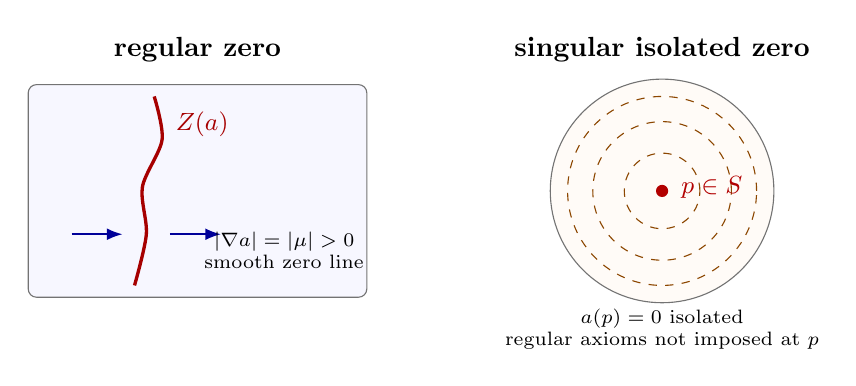
\begin{tikzpicture}[
  every node/.style={font=\small},
  grad/.style={-{Latex[length=2mm]},thick,blue!60!black}
]
  \node[font=\bfseries] at (-3.1,1.8) {regular zero};
  \draw[rounded corners=3pt,draw=black!55,fill=blue!3]
    (-5.25,-1.35) rectangle (-0.95,1.35);
  \draw[very thick,red!65!black]
    plot[smooth] coordinates {(-3.9,-1.2) (-3.75,-0.55) (-3.8,0.05)
                              (-3.55,0.65) (-3.65,1.2)};
  \node[red!65!black,anchor=west] at (-3.5,0.85) {$Z(a)$};
  \draw[grad] (-4.7,-0.55) -- (-4.05,-0.55);
  \draw[grad] (-3.45,-0.55) -- (-2.8,-0.55);
  \node[align=center,font=\scriptsize] at (-2.0,-0.75)
    {$|\nabla a|=|\mu|>0$\\smooth zero line};

  \node[font=\bfseries] at (2.8,1.8) {singular isolated zero};
  \fill[orange!3] (2.8,0) circle (1.42);
  \draw[draw=black!55] (2.8,0) circle (1.42);
  \foreach \rad in {0.48,0.88,1.2}
    {\draw[dashed,orange!55!black] (2.8,0) circle (\rad);}
  \fill[red!70!black] (2.8,0) circle (2.2pt);
  \node[anchor=west,red!70!black] at (2.92,0.05) {$p\in S$};
  \node[align=center,font=\scriptsize] at (2.8,-1.75)
    {$a(p)=0$ isolated\\regular axioms not imposed at $p$};
\end{tikzpicture}
\caption{Regular and singular zero geometry.  In a regular AES with
$\mu\ne0$, the assignment crosses zero with nonvanishing gradient, so the
interior zero germ is a smooth curve.  The radial disc model instead has an
isolated zero at its declared singular point, where the assignment is not
$C^1$ and the regular structure has no local extension.}
\label{fig:regular-versus-singular-zero}
\end{figure}

\subsection{Singular arithmetic expression spaces}

The preceding theorem makes a singular framework unavoidable if one wishes to
admit isolated or branching zeros.

\begin{definition}[Singular arithmetic expression space]\label{def:singular-aes}
A \emph{singular arithmetic expression space} is a tuple
\[
 \mathfrak E_{\mathrm{sing}}=(M,S,g,a;\mu,\lambda)
\]
with the following data:
\begin{enumerate}
\item \(M\) is a nonempty oriented smooth surface, possibly with boundary, and
      \(S\subset M\) is a closed nowhere-dense singular set;
\item \(g\) is a smooth Riemannian metric on \(M\setminus S\);
\item \(a:M\to\mathbb R\) is a specified function whose restriction to
      \(M\setminus S\) is smooth;
\item \(\mu\in\mathbb R\setminus\{0\}\), \(\lambda\in\mathbb R\), and
      \[
      (M\setminus S,g,a|_{M\setminus S};\mu,\lambda)
      \]
      is a regular AES.
\item Every \(p\in S\) is locally essential: there is no neighborhood \(U\) of
      \(p\) on which \(g|_{U\setminus S}\) and \(a|_{U\setminus S}\) admit
      smooth extensions \(\widetilde g\) and \(\widetilde a\), with
      \(\widetilde g\) nondegenerate, such that
      \((U,\widetilde g,\widetilde a;\mu,\lambda)\) is a regular AES.
\end{enumerate}
The metric or assignment may possess weaker extensions across \(S\); their precise
regularity and local behavior must be checked in each example.
\end{definition}

The set \(S\) need not consist entirely of zeros.  Nowhere density keeps the regular
locus nonempty and dense, while local essentiality prevents an arbitrary enlargement
of \(S\) by points at which the regular structure extends.  For a singular AES define
\begin{equation}\label{eq:regular-singular-zero-parts}
 Z_{\mathrm{reg}}(a)=Z(a)\cap(M\setminus S),
 \qquad
 Z_{\mathrm{sing}}(a)=Z(a)\cap S.
\end{equation}
Every point of \(Z_{\mathrm{reg}}(a)\) is a regular zero by
Theorem~\ref{thm:regular-zero-locus}; a point of
\(Z_{\mathrm{sing}}(a)\) is called singular because the regular structure is not
asserted there, even when some of the underlying data happen to extend smoothly.

\subsection{A verified isolated-zero singular model}

Let
\[
 \mathbb D=\{(\xi,\eta)\in\mathbb R^2:\xi^2+\eta^2<1\},
 \qquad
 \rho=\sqrt{\xi^2+\eta^2},
\]
and fix \(\mu,\lambda>0\).  Equip the disc with
\begin{equation}\label{eq:isolated-zero-disc-metric}
 g_{\mathbb D}
 =\frac4{\lambda^2(1-\rho^2)^2}
  \bigl(d\xi^2+d\eta^2\bigr)
\end{equation}
and define
\begin{equation}\label{eq:isolated-zero-disc-assignment}
 a_{\mathbb D}(\xi,\eta)
 =
 \begin{cases}
  \displaystyle\frac{2\mu}{\lambda}
  \frac{\rho}{1-\rho^2},&(\xi,\eta)\ne(0,0),\\[7pt]
  0,&(\xi,\eta)=(0,0).
 \end{cases}
\end{equation}

\begin{proposition}[Classification of the isolated-zero disc]\label{prop:isolated-zero-singular-model}
The tuple
\[
 (\mathbb D,\{0\},g_{\mathbb D},a_{\mathbb D};\mu,\lambda)
\]
is a singular AES with the following properties.
\begin{enumerate}
\item The metric \(g_{\mathbb D}\) extends smoothly and
      nondegenerately across the center.
\item The assignment \(a_{\mathbb D}\) is smooth on
      \(\mathbb D\setminus\{0\}\) but is not \(C^1\) at the center.
\item The punctured disc is a regular AES:
      \[
      |\nabla a_{\mathbb D}|_{g_{\mathbb D}}^2
      =\mu^2+\lambda^2a_{\mathbb D}^2.
      \]
\item Its zero decomposition is
      \[
      Z_{\mathrm{reg}}(a_{\mathbb D})=\varnothing,
      \qquad
      Z_{\mathrm{sing}}(a_{\mathbb D})=\{0\}.
      \]
\end{enumerate}
\end{proposition}

\begin{proof}
Formula \eqref{eq:isolated-zero-disc-metric} is written in Cartesian
coordinates.  Its conformal factor is a positive smooth function on all of
\(\mathbb D\), proving the first claim.

Away from the origin, \(\rho\) and hence \(a_{\mathbb D}\) are smooth.  On the
\(\xi\)-axis, however,
\[
 \frac{a_{\mathbb D}(t,0)-a_{\mathbb D}(0,0)}{t}
 =\frac{2\mu}{\lambda}
  \frac{|t|}{t(1-t^2)}.
\]
The one-sided limits are \(2\mu/\lambda\) and
\(-2\mu/\lambda\).  Thus even the partial derivative in the \(\xi\)-direction
does not exist at the center, so the assignment is not \(C^1\) there.  Moreover,
the punctured assignment tends to zero at the center, so its continuous extension
is unique.  The same calculation therefore rules out every smooth local extension
agreeing with the punctured assignment and proves that the declared singular point
is locally essential.

On the punctured disc the assignment is radial, and
\[
 \frac{da_{\mathbb D}}{d\rho}
 =\frac{2\mu}{\lambda}
  \frac{1+\rho^2}{(1-\rho^2)^2}.
\]
The inverse radial metric coefficient is
\[
 g_{\mathbb D}^{\rho\rho}
 =\frac{\lambda^2(1-\rho^2)^2}{4}.
\]
Consequently,
\begin{align*}
 |\nabla a_{\mathbb D}|_{g_{\mathbb D}}^2
 &=g_{\mathbb D}^{\rho\rho}
   \left(\frac{da_{\mathbb D}}{d\rho}\right)^2\\
 &=\mu^2\frac{(1+\rho^2)^2}{(1-\rho^2)^2}\\
 &=\mu^2+
   \lambda^2
   \left(\frac{2\mu}{\lambda}
         \frac{\rho}{1-\rho^2}\right)^2,
\end{align*}
which is the regular-AES equation on
\(\mathbb D\setminus\{0\}\).  Finally,
\(a_{\mathbb D}>0\) for \(0<\rho<1\), while its declared value at the
center is zero.  The claimed zero decomposition follows.
\end{proof}

If \(s=(2/\lambda)\operatorname{arctanh}\rho\) denotes hyperbolic distance
from the center, then
\[
 a_{\mathbb D}=\frac{\mu}{\lambda}\sinh(\lambda s).
\]
This identity describes radial propagation on the punctured regular part; it
does not repair the failure of differentiability at the center.  The metric is
regular there, while the assignment is singular.

\subsection{Two essential puncture mechanisms}

The isolated-zero disc is one of two verified mechanisms by which an essential
puncture arises; they differ in which datum degenerates.

\begin{theorem}[Two essential puncture mechanisms]
\label{thm:two-essential-puncture-mechanisms}
\begin{enumerate}
  \item \textbf{Type 1: metric extends, assignment is not $C^1$.} The disc model
  $\mathfrak E_1$ of Proposition~\ref{prop:isolated-zero-singular-model}: the
  Poincar\'e metric extends smoothly and nondegenerately across the center,
  while the assignment is continuous but not $C^1$ there, with one-sided
  directional limits $\pm 2\mu/\lambda$.  Hence $S=\{0\}$ is essential,
  $Z_{\mathrm{reg}}=\varnothing$, $Z_{\mathrm{sing}}=\{0\}$, and the punctured
  disc is metrically incomplete (the puncture is at finite distance).
  \item \textbf{Type 2: assignment extends, conformal background degenerates.}
  When the assignment $a$ extends smoothly to $\widetilde a$ on $\overline M$,
  and the metric is conformal to a smooth nondegenerate background $g_0$ on
  $U\setminus S$, the essential puncture set is exactly the critical locus:
  \[
    S=\operatorname{Crit}(\widetilde a)=\{p:d\widetilde a(p)=0\},
    \qquad
    g=\frac{|d\widetilde a|_{g_0}^2}{\mu^2+\lambda^2\widetilde a^2}\,g_0 .
  \]
  In the four-circle polynomial model the tangent cone at the origin is the
  double coordinate-axes union $(xy)^2=0$, and the zero locus is four circles
  with eight branches meeting at the puncture, the conformal factor degenerating
  like $O(|x|^{10})$ so that the puncture is at finite distance
  ($\texttt{thm:p0-punctures-are-critical}$, $\texttt{thm:p0-four-circle-model}$
  of Paper~0).
\end{enumerate}
\end{theorem}

\begin{remark}[The criticality hypothesis]
\label{rem:critical-puncture-hypothesis}
The inclusion $\operatorname{Crit}(\widetilde a)\subseteq S$ always holds when
$\widetilde a$ extends smoothly; the reverse inclusion $S\subseteq
\operatorname{Crit}(\widetilde a)$ requires the stated conformal-background
hypothesis.  Without it, a counterexample with $da\neq0$ yet singular metric at
a puncture is recorded (C-10 of the notes reserve); the two inclusions must not
be conflated.
\end{remark}

\subsection{Smooth parameter families and their total zero sets}

Let \(I\subset\mathbb R\) be an open interval, let \(M\) be a smooth
\(m\)-manifold without boundary, and let
\[
 A:M\times I\longrightarrow\mathbb R
\]
be smooth.  Write \(a_t(p)=A(p,t)\) and
\[
 \mathcal Z=A^{-1}(0)
 =\{(p,t)\in M\times I:a_t(p)=0\}.
\]

\begin{proposition}[Regular total zero set]\label{prop:regular-total-zero-set}
Assume that
\begin{equation}\label{eq:spatial-regular-family-hypothesis}
 d_pa_t\ne0
 \qquad\text{whenever }a_t(p)=0.
\end{equation}
Then \(\mathcal Z\) is a smooth embedded codimension-one submanifold of
\(M\times I\), and the restriction
\begin{equation}\label{eq:zero-family-projection}
 \pi:\mathcal Z\longrightarrow I,
 \qquad
 \pi(p,t)=t,
\end{equation}
is a submersion.  In particular, if \(\dim M=2\), then
\(\mathcal Z\) is a smooth surface.
\end{proposition}

\begin{proof}
At a point \((p,t)\in\mathcal Z\), the total differential is
\[
 dA_{(p,t)}(v,\tau)
 =d_pa_t(v)+d_tA_{(p,t)}(\tau).
\]
Hypothesis \eqref{eq:spatial-regular-family-hypothesis} implies that
\(dA_{(p,t)}\ne0\), so \(0\) is a regular value of \(A\).  The regular-value
theorem proves that \(\mathcal Z\) is a codimension-one embedded submanifold.

It remains to prove the stronger assertion about the projection.  Given an
arbitrary \(\tau\in T_tI\), put
\(c=d_tA_{(p,t)}(\tau)\), and choose \(w\in T_pM\) with
\(d_pa_t(w)=1\), which is possible because \(d_pa_t\ne0\).  Set
\[
 v=-c\,w.
\]
Then \(dA_{(p,t)}(v,\tau)=0\), so
\((v,\tau)\in T_{(p,t)}\mathcal Z\), while
\(d\pi_{(p,t)}(v,\tau)=\tau\).  Hence \(d\pi\) is surjective at every
point of \(\mathcal Z\), proving that \(\pi\) is a submersion.
\end{proof}

\begin{remark}[Properness warning]\label{rem:zero-family-properness}
Proposition~\ref{prop:regular-total-zero-set} gives pointwise product charts
for the projection, but it does not make \(\pi:\mathcal Z\to I\) a globally
trivial family, or even a fiber bundle over an entire parameter neighborhood
when noncompact fibers are present.  A standard sufficient hypothesis for local
triviality as a smooth fiber bundle is that the projection onto the relevant
parameter interval be a proper surjective submersion (with the usual additional
care if boundaries are introduced).  Without properness, components may escape
to or arrive from infinity.  Accordingly, \(\mathcal Z\) is called the
\emph{total zero set} here, not a zero tube.
\end{remark}

No multi-zero model is included in this foundational chapter.  Constructing and
classifying such models requires a complete audit of the domain, metric,
assignment, singular set, flow equation, and exact zero topology; that problem
belongs to the singular-zero theory developed after Paper~I.

\section{Theory of Caps and Interface Disks}\label{sec:theory-of-caps}
% Canonical Paper I source.

This chapter gives the ``hole'' and the ``cap'' a finite geometric carrier.  A
decorated directed acyclic network is thickened to a three-dimensional body
whose side surface carries the holes and whose interior carries the interface
disks; cutting the body along a disk exposes two caps.

\subsection{The decorated ball-and-tube thickening}

\begin{definition}[Decorated ball-and-tube thickening]
\label{def:decorated-ball-tube-thickening}
Let $G$ be a finite directed acyclic network with ordered typed external inputs
and outputs, ordered input/output slots and deterministic partial functions at
each gate, immutable sources, distinct occurrences, explicit copy/discard, and
binding records.  Forget the direction to obtain the underlying multigraph
$|G|$.  Choose, for each gate $v$, an oriented $3$-ball $B_v$ with disjoint
parametrized port disks on its boundary, one per slot; for each internal wire
$e$ choose a tube $T_e=D^2\times[0,1]$ and glue its end disks to the matching
port disks, orientation-compatibly.  The resulting body is $H_G$; the external
port disks are $E_G$, and the observed side surface is
\[
  S_G=\partial H_G\setminus\bigcup_{D\in E_G}\operatorname{int}(D).
\]
\end{definition}

This is a declared minimal thickening rule, not an intrinsic geometry forced by
the operation arity; the bare $H_G$ or $S_G$ carries no program identity.

\begin{proposition}[Local pants and no-hidden-handle genus]
\label{prop:local-pants-handlebody-genus}
\begin{enumerate}
  \item A gate with total port count three has its sphere minus the three open
  port disks a \emph{pair of pants}; total port count two gives a cylinder, one
  gives a disk.  The $2\to1$ and $1\to2$ decorations are distinct.
  \item For a connected $G$, $H_G$ is a handlebody with
  \[
    g(H_G)=\beta_1(|G|),
    \qquad
    \chi(S_G)=2-2\beta_1(|G|)-b,
  \]
  where $b=|E_G|$ is the number of external ports.
\end{enumerate}
\end{proposition}

\begin{proof}
(1) is the classification of surfaces with boundary.  (2) Assemble along a
spanning tree of $|G|$: each gate ball is a $0$-handle, each tree edge glues two
balls into one, and each remaining internal edge adds a $1$-handle; hence the
genus is the number of independent cycles.  The closed boundary of a genus-$g$
handlebody has Euler characteristic $2-2g$, and deleting $b$ open port disks
lowers it by $b$.
\end{proof}

\subsection{Interface disks and the hole--disk complementarity}

\begin{proposition}[Pants gluing along an interface disk]
\label{prop:pants-gluing-interface-disk}
Let two three-port gate balls be connected by one output--input tube.  At the
mid-section take the disk $D_e=D^2\times\{1/2\}$ and its boundary circle
$C_e=\partial D_e$.  Cutting along $D_e$ and absorbing the half-tubes into the
two collars, the two bodies are $3$-balls and the side surfaces are pants;
regluing along $D_e$ is, on the side surfaces, gluing along $C_e$:
\[
  B_1\cup_{D_e}B_2\cong B^3,
  \qquad
  S_G\cong P_1\cup_{C_e}P_2,
  \qquad
  \partial D_e=C_e .
\]
\end{proposition}

\begin{proof}
Two balls joined by one $1$-handle is again a ball (the underlying graph is a
tree); the interior disk is not part of the exposed boundary, and its circle
becomes the seam of the remaining boundary, a four-holed sphere with
$\chi=-1-1=-2$.
\end{proof}

\begin{theorem}[Hole--disk complementarity]
\label{thm:hole-disk-complementarity}
In the four-holed side surface $S_G$ and the thickened body $H_G$ of the
preceding proposition:
\begin{enumerate}
  \item \textbf{Surface non-fillability (hole).} $[C_e]\neq0\in H_1(S_G;\mathbb F_2)$:
  $C_e$ bounds no disk inside $S_G$.
  \item \textbf{Body fillability (disk/cap).} Under the inclusion
  $i:S_G\hookrightarrow H_G$, $i_*[C_e]=0\in H_1(H_G;\mathbb F_2)$, witnessed by
  the explicit disk $D_e\subset H_G$ with $\partial D_e=C_e$.
  \item \textbf{Cutting exposes caps.} Cutting $H_G$ along $D_e$ splits the single
  internal disk into two copies $D_e^+,D_e^-$ with opposite boundary
  orientations, each capping one pants opening.
\end{enumerate}
Hence the surface gives the hole its meaning and the body gives the disk its
meaning, the two being linked by the oriented common edge $C_e=\partial D_e$.
\end{theorem}

\begin{proof}
(1) and (2) are the mod-$2$ homology computation recorded and verified in
Appendix~\ref{app:pants-cellulation-verification}: the side-surface boundary
matrix has rank $110$, rising to $111$ on adjoining $C_e$, so $C_e$ is not a
boundary in $S_G$, while $C_e=\partial D_e$ is a boundary in $H_G$.  (3) is the
cut description of Proposition~\ref{prop:pants-gluing-interface-disk}.
\end{proof}

\begin{remark}[Down-set frontier disks]
\label{rem:downset-frontier-disks}
For a down-set $U\in\mathcal O(P)$ of the dependency poset of
Theorem~\ref{thm:birkhoff-downset-spinal}, cutting every internal tube that
points from $U$ to $P\setminus U$ yields the family of interface disks
$\{D_e\}_{e\in\partial^+U}$ representing the computational frontier.
\end{remark}

\subsection{The seam-circle holonomy}

The hole--disk complementarity of
Theorem~\ref{thm:hole-disk-complementarity} is topological.  It has an analytic
counterpart: the seam circle carries a holonomy of the surface potential, which
is the boundary reading of the bulk curvature of
Section~\ref{sec:differential-theory}.

\begin{definition}[Surface potential]
\label{def:surface-potential}
Let the arithmetic data $(a,v)$ be declared along the side surface $S_G$, with
$a$ the assignment and $v$ the multiplicative coordinate.  The \emph{surface
potential} is the one-form
\[
  \beta:=(-\lambda a\,dv)\big|_{S_G},
\]
the restriction to $S_G$ of the primitive $-\lambda a\,dv$ whose exterior
derivative is the contact curvature $d\alpha=-\lambda\,da\wedge dv$.
\end{definition}

\begin{proposition}[Seam-circle holonomy]
\label{prop:seam-circle-holonomy}
For the seam circle $C_e=\partial D_e$ of
Proposition~\ref{prop:pants-gluing-interface-disk}, assume that the declared
data $a,v$ extend smoothly to a neighborhood of $D_e$ and that $\lambda$ is
constant.  Write $\widetilde\beta=-\lambda a\,dv$ on that neighborhood, with
boundary restriction $\beta$.  With the induced boundary orientation, the loop integral
\[
  \oint_{C_e}\beta=\oint_{C_e}(-\lambda a\,dv)
\]
is the \emph{seam-circle holonomy}.  By the holographic Stokes theorem of
Proposition~\ref{prop:holographic-stokes-minimal}, this holonomy is the boundary
reading of the bulk curvature $\int_\Sigma d\alpha$ over the disk $\Sigma=D_e$
that fills $C_e$; hence the same circle that is topologically non-fillable in
$S_G$ ($[C_e]\neq0$) is analytically the carrier of a holonomy that the filling
disk realizes.
\end{proposition}

\begin{proof}
The first assertion is the definition.  The second is
Proposition~\ref{prop:holographic-stokes-minimal} applied to the filling disk
$\Sigma=D_e$ with boundary $\partial\Sigma=C_e$: the exactness of $d\alpha$ makes
the bulk area integral equal to the boundary holonomy.  The juxtaposition with
the topological non-fillability is Theorem~\ref{thm:hole-disk-complementarity}.
\end{proof}

\begin{remark}[The analytic thickening is a declared structure]
\label{rem:analytic-thickening-declared}
The surface potential $\beta$ is well-defined only after the arithmetic data
$(a,v)$ are declared on $S_G$; the ball-and-tube thickening of
Definition~\ref{def:decorated-ball-tube-thickening} is purely topological and
does not by itself carry $a,v$.  Extending the AES data from the bulk to the
thickened body and restricting to $S_G$ is the \emph{analytic thickening}, a
declared structure not yet constructed in general; the holonomy of
Proposition~\ref{prop:seam-circle-holonomy} is meaningful precisely under that
declaration.  This is the analytic counterpart of the observation that a bare
$S_G$ carries no program identity.
\end{remark}

\subsection{Drilling a tunnel and adding a surface handle}
\label{subsec:tunnel-handle-surgery}

The preceding construction distinguishes a circle that is unfillable on the
side surface from a disk that fills it in the body.  Drilling through the body
can change that filling relation.  We first describe the topological operation,
keeping all external port disks fixed; no arithmetic assignment is assumed.

\begin{proposition}[Two mouths and one new handle]
\label{prop:tunnel-boundary-surgery}
Let $H$ be a compact oriented $3$-manifold, let $\Sigma$ be a connected component
of $\partial H$, and mark $b$ disjoint external port disks on $\Sigma$.  Write
$S=\Sigma\setminus\bigcup_j\operatorname{int}E_j\cong S_{g,b}$.
Let a properly embedded arc have a closed tubular neighborhood
$N\cong D^2\times I$, meeting $\partial H$ exactly in its two end disks
$D_0,D_1\subset\operatorname{int}S$.  Drill out the relative interior of $N$
and round the corners.  The replacement side surface is
\[
 S'=\bigl(S\setminus(\operatorname{int}D_0\cup\operatorname{int}D_1)\bigr)
       \cup_{\partial D_0\sqcup\partial D_1}(S^1\times I),
 \qquad S'\cong S_{g+1,b}.
\]
Thus the tunnel wall becomes part of the boundary, the number of external
ports stays $b$, and $\chi(S')=\chi(S)-2$.  Attaching an oriented $3$-dimensional
$1$-handle along $D_0,D_1$ induces the same abstract surface replacement.
\end{proposition}

\begin{proof}
The two end disks cease to be boundary faces of the remaining body, whereas
the lateral boundary of $N$ becomes exposed.  Removing the two open disks
preserves connectedness and decreases Euler characteristic by two.  The
inserted annulus and its attaching circles all have Euler characteristic zero,
so they do not change that number.  The result is orientable, connected, and
has the original $b$ boundary circles.  The formula $\chi=2-2g-b$ gives
$g'=g+1$.  A $1$-handle also has two attaching disks and one lateral annulus,
which proves the last assertion.
\end{proof}

\begin{remark}[Extent of the surgery statement]
\label{rem:tunnel-scope}
A blind indentation replaces one boundary disk by another and adds no handle.
If the two mouths lie on distinct boundary components, the operation joins
those components: their genera add, rather than increasing one genus by one.
The proposition determines the boundary surface even for a knotted tunnel; it
does not classify the remaining $3$-manifold.  Removing a tunnel and attaching
material outside the body are also different operations on an embedded body.
The next product model fixes an unknotted tunnel and proves its body type
directly.
\end{remark}

\begin{proposition}[A pierced cap becomes an annulus]
\label{prop:pierced-cap-annulus}
Let $I=[0,1]$, let $D^2$ be an oriented closed round disk, and let $d^2$ be a
smaller concentric closed disk in its interior.  Set
\[
 H_0=I\times D^2,\qquad
 H_1=I\times\bigl(D^2\setminus\operatorname{int}d^2\bigr).
\]
Then $H_0$ is a $3$-ball and $H_1$ is a solid torus.  For $0<t_0<1$, put
\[
 D=\{t_0\}\times D^2,\quad C=\partial D,\quad
 d=\{t_0\}\times d^2,\quad c=\partial d,\quad
 A=D\setminus\operatorname{int}d.
\]
Give $c$ the boundary orientation of $d$, so that the inner boundary of $A$
has orientation $-c$.  As oriented chains,
\begin{equation}\label{eq:pierced-cap-chain}
 \partial D=C,\qquad \partial A=C-c.
\end{equation}
The same surviving curve $C$ satisfies
\[
 [C]=0\ \text{in }H_1(H_0;\mathbb Z),\qquad
 [C]=[c]\ne0\ \text{in }H_1(H_1;\mathbb Z)\cong\mathbb Z.
\]
In particular, $C$ bounds no disk, or integral $2$-chain, in the drilled body.
\end{proposition}

\begin{proof}
The annulus $D^2\setminus\operatorname{int}d^2$ is $S^1\times I$, hence
$H_1\cong S^1\times I^2\cong S^1\times D^2$ after rounding corners.
Subtracting the chain $d$ from $D$ gives
\eqref{eq:pierced-cap-chain}.  Retraction of the annulus onto its circular
factor, together with contraction of the first interval, is a deformation
retraction of $H_1$ onto $S^1$.  Both $C$ and $c$ map with degree one to this
circle, proving that their common class generates $H_1(H_1;\mathbb Z)$.
In $H_0$ the original disk $D$ fills $C$.
\end{proof}

\begin{remark}[Which circle still has a cap?]
\label{rem:drilled-body-meridian}
There are still disk-bounding curves on the new boundary.  If $r$ is a radial
arc joining the two boundaries of the annulus, then $I\times r$ is a properly
embedded disk in $H_1$.  Its boundary is a meridian of the remaining solid
torus, whereas $C$ represents its surviving longitudinal class.  In particular,
the inclusion $\partial H_1\hookrightarrow H_1$ has
\[
 H_1(\partial H_1;\mathbb Z)\cong\mathbb Z^2
 \longrightarrow H_1(H_1;\mathbb Z)\cong\mathbb Z
\]
with kernel generated by that meridian.  Calling a curve a ``hole boundary''
does not decide whether it has a filling disk; the body and the curve both
matter.  Nor, in general, is vanishing of a homology class by itself a
certificate of an embedded disk filling.
\end{remark}

\subsection{Double pants gluing and annular interface data}
\label{subsec:double-pants-annular-interface}

\begin{proposition}[A handle without directed feedback]
\label{prop:double-pants-dag-handle}
In the declared minimal thickening, join a $1\to2$ gate and a $2\to1$ gate
by two distinct output--input wires.  The side surface is $S_{1,2}$, obtained
by gluing two pants along two pairs of boundary circles.  The directed graph
is acyclic, while its underlying multigraph has first Betti number one.
\end{proposition}

\begin{proof}
Each pants has Euler characteristic $-1$; gluing along circles preserves their
sum $-2$, and four of the six boundary circles are consumed.  Thus $b=2$ and
$2-2g-2=-2$, giving $g=1$.  Both wires point from the first gate to the second,
so there is no directed cycle.  The underlying connected multigraph has two
vertices and two edges, giving $\beta_1=2-2+1=1$, in agreement with
Proposition~\ref{prop:local-pants-handlebody-genus}.  The first gluing connects
the two components; the second creates the handle.
\end{proof}

\begin{example}[The algebraic decoration is additional data]
\label{ex:split-merge-handle}
Declare a copy gate $\Delta(x)=(x,x)$, unary branch maps $f,g$, and a binary
merge $m$.  The corresponding computation is
\[
 x\longmapsto(f(x),g(x))\longmapsto m(f(x),g(x)),
\]
on its declared partial domain.  Unary gates only subdivide the two wires and
do not change the genus.  For $f=g=\id$ and $m(u,v)=u+v$ the output is $2x$,
so handle insertion does not by itself preserve the previous numerical
function.  The two parallel wires also show why the event reachability poset
alone is insufficient: one wire and two wires between the same two events
give the same order but different $\beta_1$.  Port incidence and multiplicity
must be retained alongside $P$ and $\mathcal O(P)$.
\end{example}

\begin{proposition}[Annular Stokes balance]
\label{prop:annular-stokes-balance}
In Proposition~\ref{prop:pierced-cap-annulus}, suppose a smooth one-form
$\widetilde\beta$ is declared on a neighborhood of $A$ in the drilled body.
Using the orientations in \eqref{eq:pierced-cap-chain},
\begin{equation}\label{eq:annular-stokes-balance}
 \oint_C\widetilde\beta-\oint_c\widetilde\beta
       =\int_A d\widetilde\beta.
\end{equation}
If $\widetilde\beta=-\lambda a\,dv$ for smooth declared data $a,v$ and constant
$\lambda$, this is the annular version of the seam-circle formula.  It requires
no extension across the removed disk.
\end{proposition}

\begin{proof}
Apply Stokes to the compact oriented annulus $A$ with boundary $C-c$.
For the specified potential, $d\widetilde\beta=-\lambda\,da\wedge dv$.
\end{proof}

\begin{remark}[Periods and the open arithmetic interface]
\label{rem:annular-interface-open}
If $d\widetilde\beta=0$, the two periods in
\eqref{eq:annular-stokes-balance} agree but need not vanish.  For example, on
the punctured disk with coordinates $(\xi,\eta)$,
\[
 \omega=\frac{-\eta\,d\xi+\xi\,d\eta}{\xi^2+\eta^2}
\]
is smooth and closed, and both positively oriented circular periods are
$2\pi$.  This is an example for a general one-form; it does not assert a
global representation of $\omega$ by arithmetic data $-\lambda a\,dv$.

Topological non-fillability neither forces a nonzero period nor assigns a
spectral value to a circle.  A proposed arithmetic annular interface must
specify both boundary state spaces and their compatibility relation, retaining
source, occurrence and production residuals.  Neither the topological surgery
nor \eqref{eq:annular-stokes-balance} supplies that relation, a regular AES
realization, or a native \texttt{Seal} rule.  These remain open under OQ-096;
the product-model calibration is recorded in
Appendix~\ref{app:pants-cellulation-verification}.
\end{remark}

\subsection{Interface state, substitution, and the spectrum}

\begin{proposition}[Polynomial interface spectrum]
\label{prop:polynomial-interface-spectrum}
In the rational-polynomial fragment, with $Q_+:z=x+y$ and $P_\times:w=zt$ glued
along the interface disk $D_z$, the substitution is the algebra homomorphism
\[
  s^*:\mathbb Q[z]\to\mathbb Q[x,y],\qquad z\mapsto x+y ,
\]
and evaluation characters satisfy $\chi_{r,s}\circ s^*=\chi_{r+s}$.  The
``spectrum value'' on the interface is the rational point $\chi_c(z)=c$ of
$\operatorname{Spec}\mathbb Q[z]$, and the relation gluing is the tensor product
(geometric fiber product)
\[
  \mathbb Q[x,y,z]/(z-x-y)\otimes_{\mathbb Q[z]}\mathbb Q[z,t,w]/(w-zt)
  \cong\mathbb Q[x,y,t,w]/(w-(x+y)t).
\]
The spectrum $\operatorname{Spec}A_z$ is a state-parameter space, not the
geometric seam circle $C_z$ and not the Stone order spectrum of
Theorem~\ref{thm:birkhoff-downset-spinal}.
\end{proposition}

\begin{proof}
Direct substitution and elimination of $z$; the choice of this model as the AEG
interface-spectrum semantics is a structural proposal, the displayed algebra
itself being a proved identity in the polynomial fragment.
\end{proof}

\begin{definition}[Interface record with residual]
\label{def:interface-record-with-residual}
An interface disk record is the five-tuple
\[
  \mathcal I_e=(D_e,C_e;\sigma_e,r_e,\beta_e),
\]
where $\sigma_e$ is the interface state under the declared observation layer,
$r_e$ is a recoverable production-process residual (together with any tangential
geometric residual), and $\beta_e$ is the port binding credential.  Numerical
equality of $\sigma_e$ does not identify two production histories ($2+3$ and
$1+4$ both carry $\sigma_e=5$).
\end{definition}

\subsection{The capping obstruction and certified sealing}

\begin{theorem}[Constant-boundary capping obstruction]
\label{thm:constant-boundary-capping-obstruction}
Let $D$ be a compact smooth disk, $g$ a smooth Riemannian metric, $a\in C^\infty(D)$,
and $\mu\ne0$, $\lambda\in\mathbb R$.  There is no data $(g,a)$ satisfying
$|da|_g^2=\mu^2+\lambda^2 a^2$ on $\operatorname{int}D$ and $a|_{\partial D}=c$
(constant).
\end{theorem}

\begin{proof}
Since $\mu^2+\lambda^2a^2\ge\mu^2>0$, one has $da\ne0$ throughout the interior.
If $a$ is nonconstant, compactness gives an interior extremum of $a$, where
$da=0$, a contradiction; if $a$ is constant, $da=0$ everywhere, also a
contradiction.
\end{proof}

\begin{corollary}[Capping dichotomy]
\label{cor:capping-dichotomy}
\begin{enumerate}
  \item An interface disk with numeric label $\sigma_e=c$ must not be realized
  as a compact regular AES disk with constant boundary assignment
  $a|_{C_e}=c$.
  \item To cap a level circle geometrically one must admit an interior critical
  point or a non-$C^1$/metric singularity (the singular category of
  Section~\ref{sec:zero-geometry}).
  \item To glue across a seam $C_e$ in the regular category, both sides must
  satisfy the two-sided smooth collar contract of Paper~0
  ($\texttt{def:p0-collar-contract}$).  Nonconstant $a|_{C_e}$ is necessary
  if a compact regular AES disk is also to fill that seam.  The disk
  obstruction alone imposes no such conclusion on gluing annular collars
  without a disk filling.
\end{enumerate}
\end{corollary}

\begin{definition}[Certified cap tuple]
\label{def:certified-cap-tuple}
A candidate \emph{certified cap} is a six-tuple
\[
  \mathcal C=(D,C,\sigma,r,w;\mathcal Q),
\]
where $D,C$ are the declared fill and its edge, $\sigma$ a state, $r$ a
residual, $w$ a verification certificate against an explicit closure obligation,
and $\mathcal Q$ the declared observation scope.  Four closure judgments are kept
distinct: (i) computational port substitution binding, (ii) topological
disk-filling $\partial D=C$ or conformal cusp filling, (iii) regular AES collar
descent or essential-singularity removal, and (iv) the Adva
\texttt{Seal \{ body \}} witness closure (additive residual zero, multiplicative
residual unit, with the non-vanishing domain obligations retained).  A
substitution success does not imply \texttt{Seal}, and $A=0,M=1$ does not by
itself produce an AES cap.
\end{definition}

\section{Conclusions and Research Interfaces}\label{sec:conclusion}
% Canonical Paper I source.
This paper has established the syntactic and projective foundation of the
programme.  The organizing principle is that an expression should not be
identified prematurely with its endpoint value.  An unmarked sequential tree
requires a choice of accumulator; the resulting fully marked planar tree is
equivalent to a bounded marked history.  From that history, operator evaluation
and the charge shadow form separate branches, while an initial value turns an
operator into an endpoint.  The non-bijective forgetful maps of
\eqref{eq:process-result-hierarchy} lose information, and the structures proved
here are the ones that survive at the syntactic and operator levels.

\subsection{Results proved here}

The first part of the paper classified binary expression trees with a unique
legal internal evaluation order and represented them by marked spinal
histories.  Operand-slot data made it possible to distinguish planar mirror,
temporal reversal, and path inverse.  These operations act at different levels
and need not induce the same operator comparison.

For nondegenerate bilateral one-hole contexts, projective continuation produced
M\"obius transformations.  The elementary contexts generate
$\operatorname{PGL}_2(K)$ over an arbitrary field, quoting the generation theorem
of Paper~0 and reading it through the history language, while ordinary addition
and nonzero scaling form the affine, or Borel, sector stabilizing the chosen
point at infinity.  This placement is important: projective semantics extends the
operator domain, but it does not turn a pole into an admissible ordinary
arithmetic operation.

The smaller alphabet consisting of translation by $\pm\sqrt2$ and negative
inversion realizes the $q=4$ Hecke group inside this projective semantics.  Its
matrix relation $(JT)^4=1$ gives an explicit pair of different marked histories
with the same operator.  The subsequent factorization through cell stabilizers
separates four levels that are needed downstream: history, operator, cell coset,
and endpoint.  In particular, arithmetic words are not identified one-to-one
with tiles in a chosen Hecke cellulation.

The second part of the paper developed the zero theory of regular arithmetic
expression spaces, using only the imported interface of
Section~\ref{sec:regular-aes-interface}.  At a zero of a regular assignment one
has $|\nabla a|=|\mu|\ne0$, so the interior zero locus is a smooth
codimension-one set and cannot have isolated points, crossings, or branch
points.  Under the additional assumptions that the metric is complete and the
manifold is connected and boundaryless, unit-gradient rectification gives the
diffeomorphism
\[
  M\cong Z(a)\times\mathbb R ,
\]
hence the zero locus is nonempty and connected.  This is not asserted for
incomplete models or manifolds with boundary, and it is not in general a
Riemannian product decomposition.  The splitting theorem is therefore a no-go
statement for branching zero networks in the regular category, and the paper
accordingly defines singular arithmetic expression spaces by a closed
nowhere-dense singular set admitting no local regular extension.  One
isolated-zero model is verified in detail; a smooth parameter family with
spatially regular zeros has a submersive total zero set, and the properness
warning records exactly how far that statement may be used.

The proved logical spine may therefore be summarized as
\[
\begin{gathered}
    \text{sequential tree}
      \longrightarrow \text{marked planar sequential tree}
      \longleftrightarrow \text{bounded marked history},\\
    \text{marked history}
      \longrightarrow \text{projective operator}
      \longrightarrow \text{ordinary endpoint or pole},\\
    \operatorname{PGL}_2
      \supset \operatorname{Aff}(1)
      \longrightarrow \text{Bruhat placement},\\
    \operatorname{Hist}_4
      \longrightarrow G_4
      \longrightarrow G_4/H_{\mathcal C}
      \longrightarrow \text{Hecke cell},\\
    \text{regular AES}
      \longrightarrow Z(a)\text{ smooth}
      \longrightarrow M\cong Z(a)\times\mathbb R \text{ when complete},\\
    \text{singular set} \longrightarrow Z_{\mathrm{reg}}(a),\,Z_{\mathrm{sing}}(a).
\end{gathered}
\]
This is a foundation for later developments, not a claim that every arithmetic
expression, singularity, or computational phenomenon is already captured by
these levels.

\subsection{What moved to Paper 0}

The geometric development that earlier versions of this paper contained is now
proved in Paper~0: the arithmetic motions of an arithmetic expression space, the
basic hyperbolic model $\mathfrak E_0$ and the punctured model
$\mathfrak E_1$, the continuous arithmetic motion and its rectification, the
point-path and ripple-pencil readings of a chronological matrix product, the
affine cocycles and the relative affine defect, the accumulative commutative
space with its weighted torsion--Stokes theorem, the reading of torsion as
tearing, and the contact structure with curvature $\mu\lambda$.  Those results
keep their labels, hypotheses, and statuses; this paper cites them and does not
maintain a second version.  The same rule now applies to the generation theorem
of \S\ref{sec:projective-affine}: its proof, and the constructive factorization
it yields, stand in Paper~0's chapter on matrix and projective unification, and
this paper keeps only the history-level statement, the affine-sector corollary,
and the Hecke sublanguage that are not developed there.  The migration is recorded in
\texttt{governance/00b-paper-0-geometric-foundation-amendment.md}.

\subsection{Interface to Paper II}

\emph{Arithmetic Expression Geometry II: Hyperbolic Real Function Theory}
begins where the horizontal connection of Paper~0 stops.  It develops additional
metric and analytic data: a horizontal metric, compatible complex or
almost-complex structures where appropriate, second-order operators,
boundary-value constructions, and arithmetic holomorphicity.  None of these
structures follows uniquely from the contact form alone, and no result of that
downstream function theory is used in the proofs of this paper
\cite{Yuan2026AEGFunctionTheory}.  The $G_4$ sublanguage supplies an additional,
explicitly arithmetic test case: an automorphic or equivariant function used
there must be derived from the group action and must keep its analytic descent
conditions separate from ordinary arithmetic admissibility of a history at a
real input.  The geometry imported by Paper~II --- the regular-AES definition,
the canonical frame, the basic model, and the contact model --- is imported from
Paper~0.

\subsection{Interface to Paper III}

\emph{Arithmetic Expression Geometry III: Singular Zero Geometry and Tubes}
studies the boundary of the regular-zero theorem.  Its objects include singular
and multiple zeros, parameter discriminants, regular and singular zero surfaces,
and tube constructions.  Braid, monodromy, and knot structures there require
separate invariance and normalization arguments.  The Hecke interface proved
here offers a source-driven alternative to imposing a four-valent cellulation by
hand: Paper~III uses a normalized Hauptmodul to construct the corresponding
singular zero dessin, then relates its sign cover to Hecke periodic-orbit knots
\cite{Yuan2026AEGZeroGeometry}.  Those analytic, singular, and three-dimensional
results remain downstream results, not results of this paper.  The complete
regular splitting theorem shows that such a branching network cannot be the zero
set of one connected, complete, boundaryless regular scalar AES; any
singularity, boundary, or incompleteness used in the construction must therefore
be stated explicitly.  In particular, the existence of a tube does not by itself
produce a knot invariant, and no such general invariant is asserted here.

\subsection{Interface to Paper IV}

\emph{Arithmetic Expression Geometry IV: Projective Condensation and
Computational Complexity} returns to the full projective process--result
hierarchy.  Its scope includes bivaluation, quotient and condensation
constructions, representation complexity, and the relation between geometric and
computational resources.  The marked-history formalism and the affine embedding
in projective semantics proved here supply an entry point, and the affine
torsion that Paper~IV compares against is the one proved in Paper~0.  Paper~IV
proves model-relative quotient and residual results together with fixed-model
resource calibrations, while general machine-robust complexity claims remain
open and require explicit models of representation, input size, and computation.

\subsection{Open foundational problems}

Several questions remain at the level of the history layer.
\begin{enumerate}
    \item Characterize the marked-history fibers of the downstream $G_4$
    operator--zero-network realization and determine what arithmetic decoration,
    if any, survives its operator and knot quotients.
    \item Produce fully verified singular multi-zero models and identify their
    stable local normal forms and discriminants; the single verified
    isolated-zero model is a starting point, not a classification.
    \item Determine when the total zero set of a parameter family is proper ---
    hence a locally trivial tube --- rather than merely a submersive family, and
    state the minimal hypotheses under which that upgrade is possible.
    \item Formulate, and then test, a quantitative relation between history
    complexity, representation complexity, and computational complexity, with an
    explicit state space, encoding, and cost model.
    \item Determine which relations among marked histories are compatible with
    ordinary admissibility, as opposed to projective non-degeneracy alone; the
    Hecke order-four example shows that the two conditions are genuinely
    different.
\end{enumerate}

These are research interfaces rather than consequences of the present paper.
The stable conclusion is narrower and more concrete: sequential arithmetic
histories possess projective operator semantics with a distinguished arithmetic
sublanguage; their affine sector is the Borel sector of that semantics; and the
regular zero geometry of an arithmetic expression space is rigid in exactly the
sense stated above, so that singular and branching phenomena require an explicit
change of category.


\section*{Acknowledgements and provenance}
\addcontentsline{toc}{section}{Acknowledgements and provenance}
The research direction, the choice of objects, and the mathematical statements
of this paper are the work of Mingli Yuan, who is the author, the corresponding
author, and the sole holder of scientific responsibility for the text.

DeepSeek Harness, an artificial-intelligence research agent running the model
\texttt{deepseek-v4-\allowbreak flash-vision-exp}, assisted with proof drafting, with
cross-checking of the finite classifications and matrix identities stated here,
with red-team reading of the claim statuses, and with the preparation of
\LaTeX{} source.  An agent is not a natural person: it cannot hold copyright,
cannot sign a transfer, and cannot correspond, so it appears on the title page
as assistance and not as a coauthor.  Contribution-level provenance, including
the commits and model identities where they are known, is maintained in
\texttt{AUTHORSHIP\_AND\_PROVENANCE.md}; the same document records the standing
rule that machine cross-checking is not independent human review.  The
mathematical statuses used here, and the boundary between proved statements and
structural proposals, are those registered in
\texttt{governance/05-mathematical-status.md}.

Under Mingli Yuan's direction, Codex (OpenAI) formalized the tunnel-drilling,
pierced-cap and double-pants arguments, the annular Stokes balance, and the
associated finite calibration, and prepared their manuscript integration.
These contributions and their verification boundaries are recorded separately
in the contribution-level provenance register.

\appendix
\section{Composition, action, and domain conventions}\label{app:conventions}
% Canonical Paper I appendix.
This appendix collects the convention-sensitive choices used in
Sections~\ref{sec:sequential-histories}--\ref{sec:projective-affine}.  The choices
are not mathematical assertions, but every composition, sign, and coordinate
formula depends on them.  The affine-group conventions that belong to the
cocycle and flow chapters of Paper~0 are collected in that paper's appendix.

\subsection{Chronological words and functional composition}

\begin{convention}[Order inside a history]
\label{conv:history-order}
A history
\[
  \gamma=(g_1,\ldots,g_n)
\]
performs $g_1$ first and $g_n$ last.  Its functional evaluation is therefore
\[
  \ev(\gamma)=g_n\circ\cdots\circ g_1
\]
when the $g_i$ are viewed as maps.
\end{convention}

\begin{convention}[Chronological concatenation]
\label{conv:chronological-concatenation}
The written product $\gamma\delta$ means first perform $\gamma$ and then
perform $\delta$.  Thus
\[
  \ev(\gamma\delta)=\ev(\delta)\circ\ev(\gamma).
\]
The notation is chronological rather than functional: the earlier process is
written on the left.
\end{convention}

For example, if $g(z)=z+\mu$ and $h(z)=qz$, then the word
$\gamma=(g,h)$ and the chronological product of the one-step histories $gh$
both act as
\[
  h\circ g(z)=qz+q\mu.
\]
The reverse chronological word $hg$ acts as $g\circ h(z)=qz+\mu$.  This
two-step check fixes the sign of their endpoint difference:
\[
  \ev(gh)(z)-\ev(hg)(z)=\mu(q-1).
\]

\subsection{Column-vector projective action}

\begin{convention}[Matrix action]
\label{conv:column-projective-action}
Homogeneous coordinates are columns, and matrices act from the left:
\[
  \begin{pmatrix}A&B\\C&D\end{pmatrix}
  \begin{pmatrix}u\\v\end{pmatrix}
  =\begin{pmatrix}Au+Bv\\Cu+Dv\end{pmatrix}.
\]
On the affine chart $z=[z:1]$, this gives
\[
  M\cdot z=\frac{Az+B}{Cz+D}.
\]
\end{convention}

If $M_i$ represents $g_i$, the history $(g_1,\ldots,g_n)$ is represented by
\[
  M_n\cdots M_1.
\]
Consequently, for chronological concatenation,
\begin{equation}
  \rho(\gamma\delta)=\rho(\delta)\rho(\gamma).
  \label{eq:appendix-rho-composition-order}
\end{equation}
This is the matrix version of
Convention~\ref{conv:chronological-concatenation}.  A row-vector right action
would require a different product convention; it is not used in this paper.

Projective matrices are scalar classes.  If $M$ and $aM$ differ by
$a\in K^\times$, they represent the same element of
$\operatorname{PGL}_2(K)$.  Matrix identities used for projective maps may
therefore be checked either exactly in $\operatorname{GL}_2(K)$ or up to one
overall nonzero scalar, provided the choice is stated.

\subsection{Ordinary and projective domains}

The following table records the domain distinction for the contexts involving
division.  Here $c\in K$ and $z$ is the evolving affine value.

\begin{center}
\renewcommand{\arraystretch}{1.35}
\begin{tabular}{llll}
\toprule
Context & Ordinary rule & Ordinary condition & Projective status \\
\midrule
$C_{/,c}^{(1)}[z]=z/c$
& divide by fixed $c$
& $c\ne0$
& invertible if $c\ne0$ \\
$C_{/,c}^{(2)}[z]=c/z$
& divide by evolving $z$
& $z\ne0$
& invertible if $c\ne0$ \\
$C_{\times,c}^{(\varepsilon)}[z]=cz$
& multiply by $c$
& none
& invertible if $c\ne0$ \\
\bottomrule
\end{tabular}
\end{center}

Two different exclusions appear in the table.  The parameter condition
$c\ne0$ ensures that the context has an invertible projective matrix.  The
state condition $z\ne0$ ensures that an ordinary second-slot division is
defined at that step.  Projectively, a non-degenerate $c/z$ sends $0$ to
$\infty$; this is a chart transition, not an ordinary quotient in $K$.

For a composite history, ordinary admissibility is checked at every
intermediate state.  It is not enough that the final projective point lies in
the affine chart.  In particular, two projective inversions compose to the
identity operator, but the corresponding ordinary two-step word is not
admissible at zero.

\subsection{Mirror, reversal, and inverse notation}

For $\gamma=(g_1,\ldots,g_n)$, the three operations are summarized by
\begin{center}
\begin{tabular}{lll}
\toprule
Operation & Resulting word & Required hypothesis \\
\midrule
Mirror $m\gamma$
& $(m(g_1),\ldots,m(g_n))$
& none \\
Temporal reversal $r\gamma$
& $(g_n,\ldots,g_1)$
& none \\
Path inverse $\gamma^{-1}$
& $(g_n^{-1},\ldots,g_1^{-1})$
& every $g_i$ invertible \\
\bottomrule
\end{tabular}
\end{center}
Mirror exchanges operand slots and retains time.  Temporal reversal changes
time and retains the original contexts.  Path inverse reverses time and
inverts every operator.  Accordingly,
\[
  \rho(\gamma^{-1})=\rho(\gamma)^{-1},
\]
whereas no analogous identity holds for $r\gamma$ in general.

\subsection{Notation conversion summary}

The table below lists older or potentially ambiguous descriptions and the
notation used in Paper~I.

\begin{center}
\renewcommand{\arraystretch}{1.25}
\begin{tabular}{ll}
\toprule
Potentially ambiguous description & Paper~I notation \\
\midrule
evolving value in operand slot one
& $C_{\omega,c}^{(1)}[z]=\omega(z,c)$ \\
evolving value in operand slot two
& $C_{\omega,c}^{(2)}[z]=\omega(c,z)$ \\
chronological context word
& $\gamma=(g_1,\ldots,g_n)$, $g_1$ first \\
history product
& $\gamma\delta$, first $\gamma$, then $\delta$ \\
operator evaluation
& $\rho(\gamma)$ \\
ordinary endpoint at $x$
& $\nu_x(\gamma)$ \\
operand-slot exchange
& $m\gamma$ \\
time-order reversal
& $r\gamma$ \\
inverse operator path
& $\gamma^{-1}$ \\
\bottomrule
\end{tabular}
\end{center}

\section{Equality and elementary neutrality examples}\label{app:equality-neutrality}
% Canonical Paper I appendix.
The examples below separate several equality tests without developing a general
relation or loop theory.  In each case, histories are marked chronological
words, operators are affine maps, and endpoint values are obtained only after
choosing an input.

Two step families are used throughout, with the notation and the parameters
of Paper~0:
\[
  \mathsf A_p(z)=z+p,
  \qquad
  \mathsf M_q(z)=e^{q}z,
  \qquad p,q\in\mathbb R .
\]
Negative \(p\) and \(q\) are allowed, so the same notation covers inverse
translations and inverse positive scalings.  For a word \(\gamma\) of these
steps we write \(A_\gamma=\sum_i p_i\) and \(M_\gamma=\sum_i q_i\) for its
two totals.  Paper~0 constructs the space of which the pair
\((A_\gamma,M_\gamma)\) is the endpoint, proves that this endpoint is the
abelianization of the history group, and proves the theorems that measure the
order defect of two histories with equal totals; none of those theorems is
restated here.  The totals are used below only as bookkeeping, to say exactly
what a pair of totals retains and what it forgets.

\subsection{Same value, different operators}

Let
\[
    \gamma=(\mathsf A_1),
    \qquad
    \delta=(\mathsf M_{\log 2}).
\]
At the input \(x=1\), both histories have endpoint value \(2\).  Their induced
operators are nevertheless
\[
    \nu_x(\gamma)=x+1,
    \qquad
    \nu_x(\delta)=2x,
\]
which are unequal.  Equality at one input therefore does not imply operator
equality.

\subsection{Same operator, different histories}

The marked histories
\[
    \gamma=(\mathsf A_1,\mathsf A_2),
    \qquad
    \delta=(\mathsf A_2,\mathsf A_1)
\]
are different chronological words, but both induce \(x\mapsto x+3\).  They
also have the same totals, \(A_\gamma=A_\delta=3\) and
\(M_\gamma=M_\delta=0\).  Thus operator equality does not recover a marked
history, even when the totals are retained.

\subsection{Neutral endpoint, nontrivial history}

For \(p\ne0\), the nonempty history
\[
    \ell=(\mathsf A_p,\mathsf A_{-p})
\]
induces the identity operator and hence has zero endpoint defect for every
input.  It is nevertheless not the empty marked history.  In particular,
operator neutrality does not imply literal or historical equality.

A slightly different phenomenon occurs for
\[
    \gamma=(\mathsf A_p,\mathsf M_q,\mathsf A_{-p},\mathsf M_{-q}),
    \qquad p,q\ne0 .
\]
Its totals vanish, \(A_\gamma=0\) and \(M_\gamma=0\), but it induces the
translation
\[
    z\longmapsto z+p(1-e^{-q}),
\]
which is not the identity.  Thus vanishing totals do not imply operator
neutrality, even though the individual steps are all non-degenerate and
ordinarily admissible on an open set.

These examples exhibit the hierarchy needed in the main text:
\[
    \text{marked history}
      \longrightarrow \text{operator}
      \longrightarrow \text{endpoint value},
\]
with the two totals providing an additional, order-forgetting projection.  No
converse implication between adjacent levels holds in general.

Two further separations belong to Paper~0 and are not repeated here: histories
with equal totals but nonzero relative defect, and the distinction between the
open two-step defect and the closed-loop drift of the same word.  They are
proved there as the relative torsion of two charge-compatible histories and as
the finite comparison of the two orders, in the chapters on the accumulative
commutative space and on the contact model, and their computations are
collected in Paper~0's appendices on affine cocycles and on the ACS and contact
calculations.

\section{Symbolic verification of the Magnus series and PBW abelianization}\label{app:magnus-verification}
% Canonical Paper I appendix.

This appendix records the symbolic verification of the Magnus-series low-order
terms of Definition~\ref{def:history-magnus-series} and the PBW abelianization
of Theorem~\ref{thm:pbw-abelianization-difference-substitution}.

\subsection{The order-three free nilpotent matrix model}

Work in the free order-three nilpotent Lie algebra $\mathfrak n_4$ of strictly
upper-triangular $4\times4$ matrices, realized by the elementary matrices
\[
  X=E_{12},\qquad Y=E_{23},\qquad Z=E_{34},
\]
whose only nonzero products are $XY=E_{13}$, $YZ=E_{24}$, $XYZ=E_{14}$; all
brackets of depth four or more vanish.  The relevant brackets are
\[
  [X,Y]=E_{13},\qquad [Y,Z]=E_{24},\qquad [X,[Y,Z]]=[Z,[X,Y]]=E_{14},\qquad
  [Y,[Z,X]]=0 .
\]

\subsection{Symbolic expansion to order three}

For scalar parameters $h,k,l$, form the truncated exponentials
\[
  e^{hX}=I+hX+\tfrac{h^2}{2}X^2+\tfrac{h^3}{6}X^3,
\]
and similarly for $Y,Z$; here $X^2=0$ in the present model, so the exponential
is a polynomial.  The chronological product $e^{lZ}e^{kY}e^{hX}$ has formal
logarithm obtained from the series $\log(I+T)=T-\tfrac12T^2+\tfrac13T^3$, with
$T=e^{lZ}e^{kY}e^{hX}-I$.  The nonzero upper-triangular entries are
\[
  \Omega_{12}=h,\qquad
  \Omega_{23}=k,\qquad
  \Omega_{34}=l,\qquad
  \Omega_{13}=\tfrac12hk,\qquad
  \Omega_{24}=\tfrac12kl,\qquad
  \Omega_{14}=\tfrac13hkl .
\]
These are the coefficients claimed in
Proposition~\ref{prop:arity-cell-correspondence-low-order}: the order-one terms
$h,k,l$ are the arity-$1$ charges, the order-two terms $\tfrac12hk,\tfrac12kl$
are the arity-$2$ commutators $[X,Y],[Y,Z]$, and the order-three term
$\tfrac13hkl$ is the arity-$3$ bracket $[X,[Y,Z]]$.  The repeated-generator
self-nesting terms $[X,[X,Y]]$ and $[Y,[X,Y]]$ vanish in $\mathfrak n_4$ because
$X^2=Y^2=0$; they are nonzero only in a step-$3$ model with nonzero squares,
which is not needed for the low-order arity correspondence.

\subsection{PBW abelianization check}

Setting all brackets to zero abelianizes $\mathfrak L$: the bracket monomials
$[X,Y]\mapsto0$, $[X,[Y,Z]]\mapsto0$, and the Magnus series degenerates to the
abelian sum
\[
  \Omega(\gamma)\mapsto hX+kY+lZ,
\]
whose coefficient vector $(h,k,l)$ is the cumulative sum of the increments ---
the abelian form of the difference substitution of
Theorem~\ref{thm:pbw-abelianization-difference-substitution}.  Under the PBW
filtration, the word $ZYX$ (i.e.\ $Z\otimes Y\otimes X$) has associated graded
the monomial $XYZ$ in the symmetric algebra $S(\mathfrak L)$, which is the
commutative degeneration of the Lyndon word $[X,[Y,Z]]$ together with the
abelian part.

\section{Finite cellulation and mod-2 homology verification for pants gluing}\label{app:pants-cellulation-verification}
% Canonical Paper I appendix.

This appendix records the finite cellulation and mod-2 homology verification of
Theorem~\ref{thm:hole-disk-complementarity} (V1 of OQ-096).

\subsection{The V1 finite model}

Two solid boxes $[0,3]^3$ and $[5,8]\times[0,3]^2$ model two three-port gates,
joined by the connecting tube $[3,5]\times[1,2]^2$.  The cellulation has $56$
unit cubes, $336$ tetrahedra, and $132$ vertices.  Every vertex link was checked
for being a disk or a sphere ($116$ disks, $16$ spheres), establishing the
local manifoldness of the thickened body.

\subsection{Surface and body homology data}

The two pants side surfaces each have $(V,E,F)=(60,116,55)$ with three boundary
circles; the glued side surface has $(V,E,F)=(116,228,110)$ with four boundary
circles and Euler characteristic $\chi=-2$, matching
Proposition~\ref{prop:local-pants-handlebody-genus} ($\beta_1=0$, $b=4$).  The
shared interface disk is one square; its four oriented edges form the seam
circle $C$, with opposite orientation on the two sides.

The mod-2 side-surface boundary matrix has rank $110$; adjoining the chain $C$
raises the rank to $111$, proving
$[C]\neq0\in H_1(S_G;\mathbb F_2)$.  In the body, the explicit disk gives
$\partial D=C$, so $i_*[C]=0\in H_1(H_G;\mathbb F_2)$.

\subsection{Negative controls}

Ten negative controls were executed and all rejected: a control is accepted only
if it violates a declared condition (wrong orientation, a non-manifold link, a
mismatched boundary count, or a spurious disk filling in the side surface).
The substitution $z=x+y$, $w=zt$ at $(x,y,t)=(2,3,4)$ gives interface value $5$
and output $20$ by exact rational arithmetic, agreeing with the graph binding.

\subsection{Status}

This is a \emph{computationally verified example} for a single fixed model.  The
construction and the checker are by the same author; it does not close the
general composition, the AES-extension, or the native \texttt{Seal} bridge
obligations (V2--V4 of OQ-096).

\subsection{Product-tunnel calibration}
\label{app:product-tunnel-calibration}

The successor \path{research/pants-interface-disks/verify_handles.py} checks
the fixed cubical version of Proposition~\ref{prop:pierced-cap-annulus}.
Start with $[0,3]^3$.  Removing only the cube with lower corner $(0,1,1)$
makes a blind indentation; removing all three cubes with lower corners
$(j,1,1)$, $j=0,1,2$, makes a through tunnel.  The interface is the square
$D=\{1\}\times[0,3]^2$, with outer boundary $C$, and its removed central
square has boundary $c$.  The surviving eight faces form the annulus $A$.

\begin{center}
\begin{tabular}{lrrrr}
\toprule
Body & Cubes & $\chi(H)$ & $\chi(\partial H)$ & $b_1(H;\mathbb F_2)$\\
\midrule
Solid box & 27 & 1 & 2 & 0\\
Blind indentation & 26 & 1 & 2 & 0\\
Through tunnel & 24 & 0 & 0 & 1\\
\bottomrule
\end{tabular}
\end{center}

The checker verifies face incidences, boundary orientability and connectedness,
and all $64$ vertex links in each body.  The solid box has $56$ disk and $8$
sphere links, the indentation $60$ disk and $4$ sphere links, and the tunnel
$64$ disk links.  The tunnel boundary has $64$ vertices, $192$ edges and
$128$ triangles.  These local checks supplement the product-model proof;
Euler characteristic alone is not used to identify a $3$-manifold.

The body boundary map $\partial_2$ has rank $81$ for the box and $80$ for the
tunnel.  Adjoining $C$ leaves rank $81$ in the former and raises $80$ to $81$
in the latter.  Thus $C$ changes from bounding to nonbounding over
$\mathbb F_2$.  The inner circle $c$ is also nonbounding in the tunnel, while
the explicit radial rectangle gives a meridian disk.  The exact oriented-chain
check is $\partial A=C-c$.  For $\widetilde\beta=-y\,dz$, exact edge integrals
give
\[
 \oint_C\widetilde\beta=-9,\qquad
 \oint_c\widetilde\beta=-1,\qquad
 \int_A d\widetilde\beta=-8,
\]
checking the sign of Proposition~\ref{prop:annular-stokes-balance}.

Eight negative controls reject a blind pit labelled as a handle, a tunnel
labelled as a ball, survival of the removed disk, a false filling claim for
$C$, the wrong inner-boundary sign, a false zero-curvature period equality,
a missing annular face, and a vertex-only contact.  Normal and optimized Python
outputs reproduce \path{research/pants-interface-disks/evidence-handles.json}.
This is a same-author finite calibration using the V1 helper routines, not an
independent verifier or an AES/Adva realization.  It supplements the in-paper
proofs and does not discharge the annular state-compatibility problem.


\bibliographystyle{plain}
\bibliography{aeg-paper-1}
\end{document}
